\documentclass[12pt]{article}
\usepackage[left=2cm, right=2cm, top=2cm]{geometry}
\usepackage[utf8]{inputenc} 
\usepackage{graphicx} % to include images
\usepackage{amsmath} % For math mode
\usepackage{caption} % For captions
\usepackage{subcaption} % To use caption while using mini page
\usepackage{amssymb} % To use math symbols
\usepackage{multirow} %To combine multiple rows in a table
\usepackage[table]{xcolor} %To color rows / columns in table
\usepackage{titling} %To vertically center the title page
\usepackage{hyperref} %for URL


%----------------------------MATLAB TEMPLATE -------------------------------------
\usepackage{listings}
\usepackage{color} %red, green, blue, yellow, cyan, magenta, black, white
\definecolor{mygreen}{RGB}{28,172,0} % color values Red, Green, Blue
\definecolor{mylilas}{RGB}{170,55,241}
%-----------------------------------------------------------------------------------------

\title{ECE 8540 \\ Analysis of Tracking Systems \\ 
	Assignment 4}
\author{Vivek Koodli Udupa \\ C12768888}
\date{October - 09, 2018 }

%To make the title page center vertically centered
\renewcommand\maketitlehooka{\null\mbox{}\vfill}
\renewcommand\maketitlehookd{\vfill\null}

\begin{document}

%Displaying Title
\begin{titlepage}
\maketitle
\pagenumbering{gobble}% Remove page numbers (and reset to 1)
\end{titlepage}
\pagenumbering{arabic}% Arabic page numbers (and reset to 1)


%Begin of Report

\section{Introduction}
In this report we consider the problem of filtering; Kalman filtering to be specific. Filtering is a method of mitigating noise in sensor data. A set of sensor data is used to design a model. The model can be used to smooth out the noise and to make prediction about expected future states. However, in the case of tracking problem, the thing that is to be tracked is not expected to follow a linear predictable behavior all the time. If the object did follow a predictable path, then there would be no point in tracking it. In such a situation, the behavior of the object could just be modeled perfectly and the future behavior is completely known.  \\
\\
For example, Consider the problem of tracking a bullet fired through some kind of gun. Initially the bullet travels straight, but as time progresses, the bullet is slowed down due to gravity, air resistance and multiple other factors and its trajectory changes. Thus the bullet follows certain path for a particular duration and then changes its path for the next set period of time. In order to track such an object, that changes behavior slowly but continuously, it is necessary to change the model fit continuously. In the extreme this leads to the concept of updating the model fit after every new sensor reading is recorded. This is how filtering works. \\
\\
In the problem of tracking something, we are trying to find the answer for the question \lq\lq{} where is the object? \rq\rq{}. The answer to this question is rarely if ever certain in real life applications. The answer is mostly a probability distribution of \lq\lq{} the object is likely to be in this area \rq\rq{}. This is because of the uncertainties in the sensor measurement, object's behavior and other noises that might persist. In this report we will consider data that contains dynamic and measurement noises and we will use Kalman filtering to generate predictions. Kalman filtering is an algorithm that uses a set of measurements collected over time, that contains statistical noises and other inaccuracies and produces estimates of unknown variables that tend to be more accurate than those based on single measurement alone, by estimating a joint probability distribution over the variables for each time frame.\\
\\
This report deals with the application of kalman filter to track the position of an object in both 1D and 2D space. This report starts with the visual analysis of dataset, building the kalman filter equations and then finally discussing the results of the derived kalman filter.

\section{Methods}
Kalman filter is a continuous cycle of predict and update. When formulating a problem for the Kalman filter, we consider the following steps: 

\begin{enumerate}
	\item Determine the state variables. Here we are answering the question \lq\lq{}what are we tracking?\rq\rq{}.
	\item Write the state transition equations i.e. How things evolve over time.
	\item Define the dynamic noise(s).  This describes the uncertainties in state transition equation.
	\item Determine the observation variables i.e. Sensor readings.
	\item Write the observation equations (relating the sensor readings to the state variables).
	\item Define the measurement noise(s). These are the uncertainties in observation variables.
	\item Characterize the state transition matrix and observation matrix.
	\item Check all matrices in the Kalman filter equations to make sure the sizes are appropriate.
\end{enumerate} 

\subsection{ Deriving the equations for 1D Model}
\label{sec:1D}
We will begin by describing the things that we are tracking. The state $X_t$ can be defined as: 
\begin{equation}
X_t = 
\begin{bmatrix}
	x_t \\
	\dot{x}_t
\end{bmatrix}
\label{eq:1d state}
\end{equation}
where $x_t$ is the position and $\dot{x}_t$ is the velocity. \\
\\
The second step is to write the state transition equations that describe the expected behavior of the state variables. Here, we are considering a constant 1D velocity model. The state transition equations for the model are as follows: 
\begin{align}
\begin{split}
	X_{t+1} &= x_t + T \dot{x_t} \\
	\\
	\dot{X_t} &=  \dot{x_t}
\end{split}
\label{eq:1d state transition}
\end{align}
\\
The third step is to define the dynamic noise(s). Here we will assume that random accelerations can happen between sensor samples. 
\begin{equation}
\text{dynamic noise} = 
\begin{bmatrix}
	0 \\
	N(0,\sigma^2_{a1})
\end{bmatrix}
\label{eq:1d dyn noise}
\end{equation}
Notice that the first element of the matrix is zero. The zero indicates that there is no noise in the position of the reading. Noise in position reading would indicate that the object is teleporting.  \\
\\
The forth step is to list the observation variables. Here, we are sensing the x position. Denoting the sensor reading for this as follows: 
\begin{equation}
Y_t = 
\begin{bmatrix}
	\tilde{x_t} \\
	0
\end{bmatrix}
\label{eq:1d obs var}
\end{equation}
The second element of the matrix is zero because the velocity is not being measured. \\
\\
The fifth step is to describe the observation equation.
\begin{equation}
\tilde{x_t} = x_t
\label{eq:1d obs eq}
\end{equation}
\\
The sixth step is to define measurement noise(s). Here, we will assume that the sensor reading is corrupted by noise.
\begin{equation}
\text{measurement noise} = 
\begin{bmatrix}
	N(0,\sigma^2_{n1})
\end{bmatrix}
\label{eq:1d mes noise}
\end{equation}
\\
The seventh step is to characterize the co-variance matrices. There are three of them.  \\
The co-variance of the state variables is written as:
\begin{equation}
s_t = 
\begin{bmatrix}
	\sigma^2_{x_t} & \sigma_{x_t,\dot{x_t}} \\
	\sigma_{x_t,\dot{x_t}} & \sigma^2_{\dot{x_t}}
\end{bmatrix}
\label{eq:1d state co-var}
\end{equation}
\\
Co-variance of dynamic noise can be written as:
\begin{equation}
Q = 
\begin{bmatrix}
	0 & 0 \\
	0 & \sigma^2_{a_1}
\end{bmatrix}
\label{eq:1d dyn co-var}
\end{equation}

Co-variance of measurement noise can be written as:
\begin{equation}
R = 
\begin{bmatrix}
	\sigma^2_{n_1} & 0 \\
	0 & 0
\end{bmatrix}
\label{eq:1d mes co-var}
\end{equation}
\\
The eighth step is to define the state transition and observation matrices. The state transition matrix can be obtained from equation \ref{eq:1d state transition}.
\begin{equation}
\phi = 
\begin{bmatrix}
	1 & T \\
	0 & 1
\end{bmatrix}
\label{eq:1d state trans mat}
\end{equation}
\\
The observation matrix can be obtained from equation \ref{eq:1d obs var}.
\begin{equation}
M = 
\begin{bmatrix}
	1 & 0 \\
	0 & 0
\end{bmatrix}
\label{eq:1d state trans mat}
\end{equation}
\\
Note that we have just finished formulating the 1D model for filtering problem. This is just a theoretical model of how we expect the system being tracked to behave. Implementation will be explained in section \ref{sec:implementation}

\subsection{Deriving the equations for 2D Model}
\label{sec:2D}
Similar to the derivation shown in section \ref{sec:1D} this section will show the derivation to a constant 2D velocity model. \\
We will begin by describing the things that we are tracking. The state $X_t$ can be defined as: 
\begin{equation}
X_t = 
\begin{bmatrix}
	x_t \\
	y_t \\
	\dot{x}_t\\
	\dot{y}_t
\end{bmatrix}
\label{eq:2d state}
\end{equation}
where $x_t$ and $y_t$ is the position and $\dot{x}_t$ and $\dot{y}_t$ is the velocity. \\
\\
The second step is to write the state transition equations that describe the expected behavior of the state variables. Here, we are considering a constant 2D velocity model. The state transition equations for the model are as follows: 
\begin{align}
\begin{split}
	X_{t+1} &= x_t + T \dot{x_t} \\
	\\
	Y_{t+1} &= y_t + T \dot{y_t} \\
	\\
	\dot{X_t} &=  \dot{x_t} \\
	\\
	\dot{Y_t} &=  \dot{y_t}
\end{split}
\label{eq:2d state transition}
\end{align}
\\
The third step is to define the dynamic noise(s). Here we will assume that random accelerations can happen between sensor samples. 
\begin{equation}
\text{dynamic noise} = 
\begin{bmatrix}
	0 \\
	0 \\
	N(0,\sigma^2_{a1}) \\
	N(0,\sigma^2_{a2})
\end{bmatrix}
\label{eq:2d dyn noise}
\end{equation}
\\
The forth step is to list the observation variables. Here, we are sensing the x and y positions. Denoting the sensor reading for this as follows: 
\begin{equation}
Y_t = 
\begin{bmatrix}
	\tilde{x_t} \\
	\tilde{y_t}
\end{bmatrix}
\label{eq:2d obs var}
\end{equation}
\\
The fifth step is to describe the observation equation.
\begin{align}
\begin{split}
	\tilde{x_t} = x_t \\
	\tilde{y_t} = y_t
\end{split}
\label{eq:2d obs eq}
\end{align}
\\
The sixth step is to define measurement noise(s). Here, we will assume that the sensor reading is corrupted by noise.
\begin{equation}
\text{measurement noise} = 
\begin{bmatrix}
	N(0,\sigma^2_{n1}) \\
	N(0,\sigma^2_{n2})
\end{bmatrix}
\label{eq:2d mes noise}
\end{equation}
\\
The seventh step is to characterize the co-variance matrices. There are three of them.  \\
The co-variance of the state variables is written as:
\begin{equation}
s_t = 
\begin{bmatrix}
	\sigma^2_{x_t} & \sigma_{x_t,y_t} & \sigma_{x_t,\dot{x_t}} & \sigma_{x_t,\dot{y_t}}  \\
	\sigma_{x_t,y_t} & \sigma^2_{y_t} & \sigma_{y_t,\dot{x_t}} & \sigma_{y_t,\dot{y_t}} \\
	\sigma_{x_t,\dot{x_t}} & \sigma_{y_t,\dot{x_t}} & \sigma^2_{\dot{x_t}} & \sigma_{\dot{x_t},\dot{y_t}} \\
	\sigma_{x_t,\dot{y_t}} & \sigma_{y_t,\dot{y_t}} & \sigma_{\dot{x_t},\dot{y_t}} & \sigma^2_{\dot{y_t}}
\end{bmatrix}
\label{eq:2d state co-var}
\end{equation}
\\
Co-variance of dynamic noise can be written as:
\begin{equation}
Q = 
\begin{bmatrix}
	0 & 0 & 0 & 0\\
	0 & 0 & 0 & 0\\
	0 & 0 & \sigma^2_{a_1} & \sigma_{a_1,a_2} \\
	0 & 0 & \sigma_{a_1,a_2} & \sigma^2_{a_2}
\end{bmatrix}
\label{eq:2d dyn co-var}
\end{equation}
\\
Co-variance of measurement noise can be written as:
\begin{equation}
R = 
\begin{bmatrix}
	\sigma^2_{n_1} & \sigma_{n_1,n_2} \\
	\sigma_{n_1,n_2} & \sigma^2_{n_2} 
\end{bmatrix}
\label{eq:2d mes co-var}
\end{equation}
\\
The eighth step is to define the state transition and observation matrices. The state transition matrix can be obtained from equation \ref{eq:2d state transition}.
\begin{equation}
\phi = 
\begin{bmatrix}
	1 & 0 & T & 0 \\
	0 & 1 & 0 & T \\
	0 & 0 & 1 & 0 \\
	0 & 0 & 0 & 1
\end{bmatrix}
\label{eq:2d state trans mat}
\end{equation}
\\
The observation matrix can be obtained from equation \ref{eq:2d obs var}.
\begin{equation}
M = 
\begin{bmatrix}
	1 & 0 & 0 & 0 \\
	0 & 1 & 0 & 0
\end{bmatrix}
\label{eq:1d state trans mat}
\end{equation}
\\
Note that we have just finished formulating the 2D model for filtering problem. This is just a theoretical model of how we expect the system being tracked to behave. Implementation will be explained in section \ref{sec:implementation}

\subsection{Implementation}
\label{sec:implementation}
As mentioned previously in section \ref{sec:1D} and section \ref{sec:2D} the Kalman filter is a continuous predict and update loop and the equations for Kalman parameters have been derived. This section will describe the implementation of this filter using the equations for the main loop.\\
\\
The equation for predicting the next state is given by:
\begin{equation}
	X_{t,t-1} = \phi\  X_{t-1,t-1}
\label{eq:imp predict}
\end{equation}
Here $X_{t,t-1}$ represents the next state based on the previous state. $\phi$ is the state transition matrix and $X_{t-1,t-1}$ is the previous state.
\\
Predicting the next state co-variance as:
\begin{equation}
	S_{t,t-1} = \phi\  S_{t-1,t-1}\ \phi^T + Q
\label{eq:imp predict state co-var}
\end{equation}
\\
Then obtain the measurements, i.e $Y_t$ \\
\\
Next, calculate the Kalman gain(weights) as:
\begin{equation}
	K_t = S_{t,t-1}\ M^T\ [\ M\ S_{t,t-1}\ M^T + R\ ]^{-1}
\label{eq:imp kalman gain}
\end{equation}
\\
Now using the predicted state, Kalman gain and measurements update the state as:
\begin{equation}
	X_{t,t} = X_{t,t-1} + K_t\ (\ Y_t\ - M\ X_{t,t-1}\ )
\label{eq:imp state update}
\end{equation}
\\
Now update the state co-variance as :
\begin{equation}
	S_{t,t} = [\ I\ -\ K_t\ M\ ]\ S_{t,t-1}
\label{eq:imp state co-var update}
\end{equation}
\\
The implementation of the above described models and equations are done in MATLAB. Please refer the Appendix for the code.  


\section{Results}
In this section we will plot the given dataset and the Kalman fiter's predicted values and see the effect of changing the measurement noise to dynamic noise ratio.\\
\\
Here we are keeping the measurement noise,R fixed at 1 and we change the dynamic noise for 1D constant velocity model.  \\
For the 2D constant velocity model we keep the dynamic noise,Q fixed at 0.01 and we change the measurement noise. \\

%Ratio 1 1:1
\begin{figure}[h]
\centering
\begin{minipage}{0.5\textwidth}
\centering
	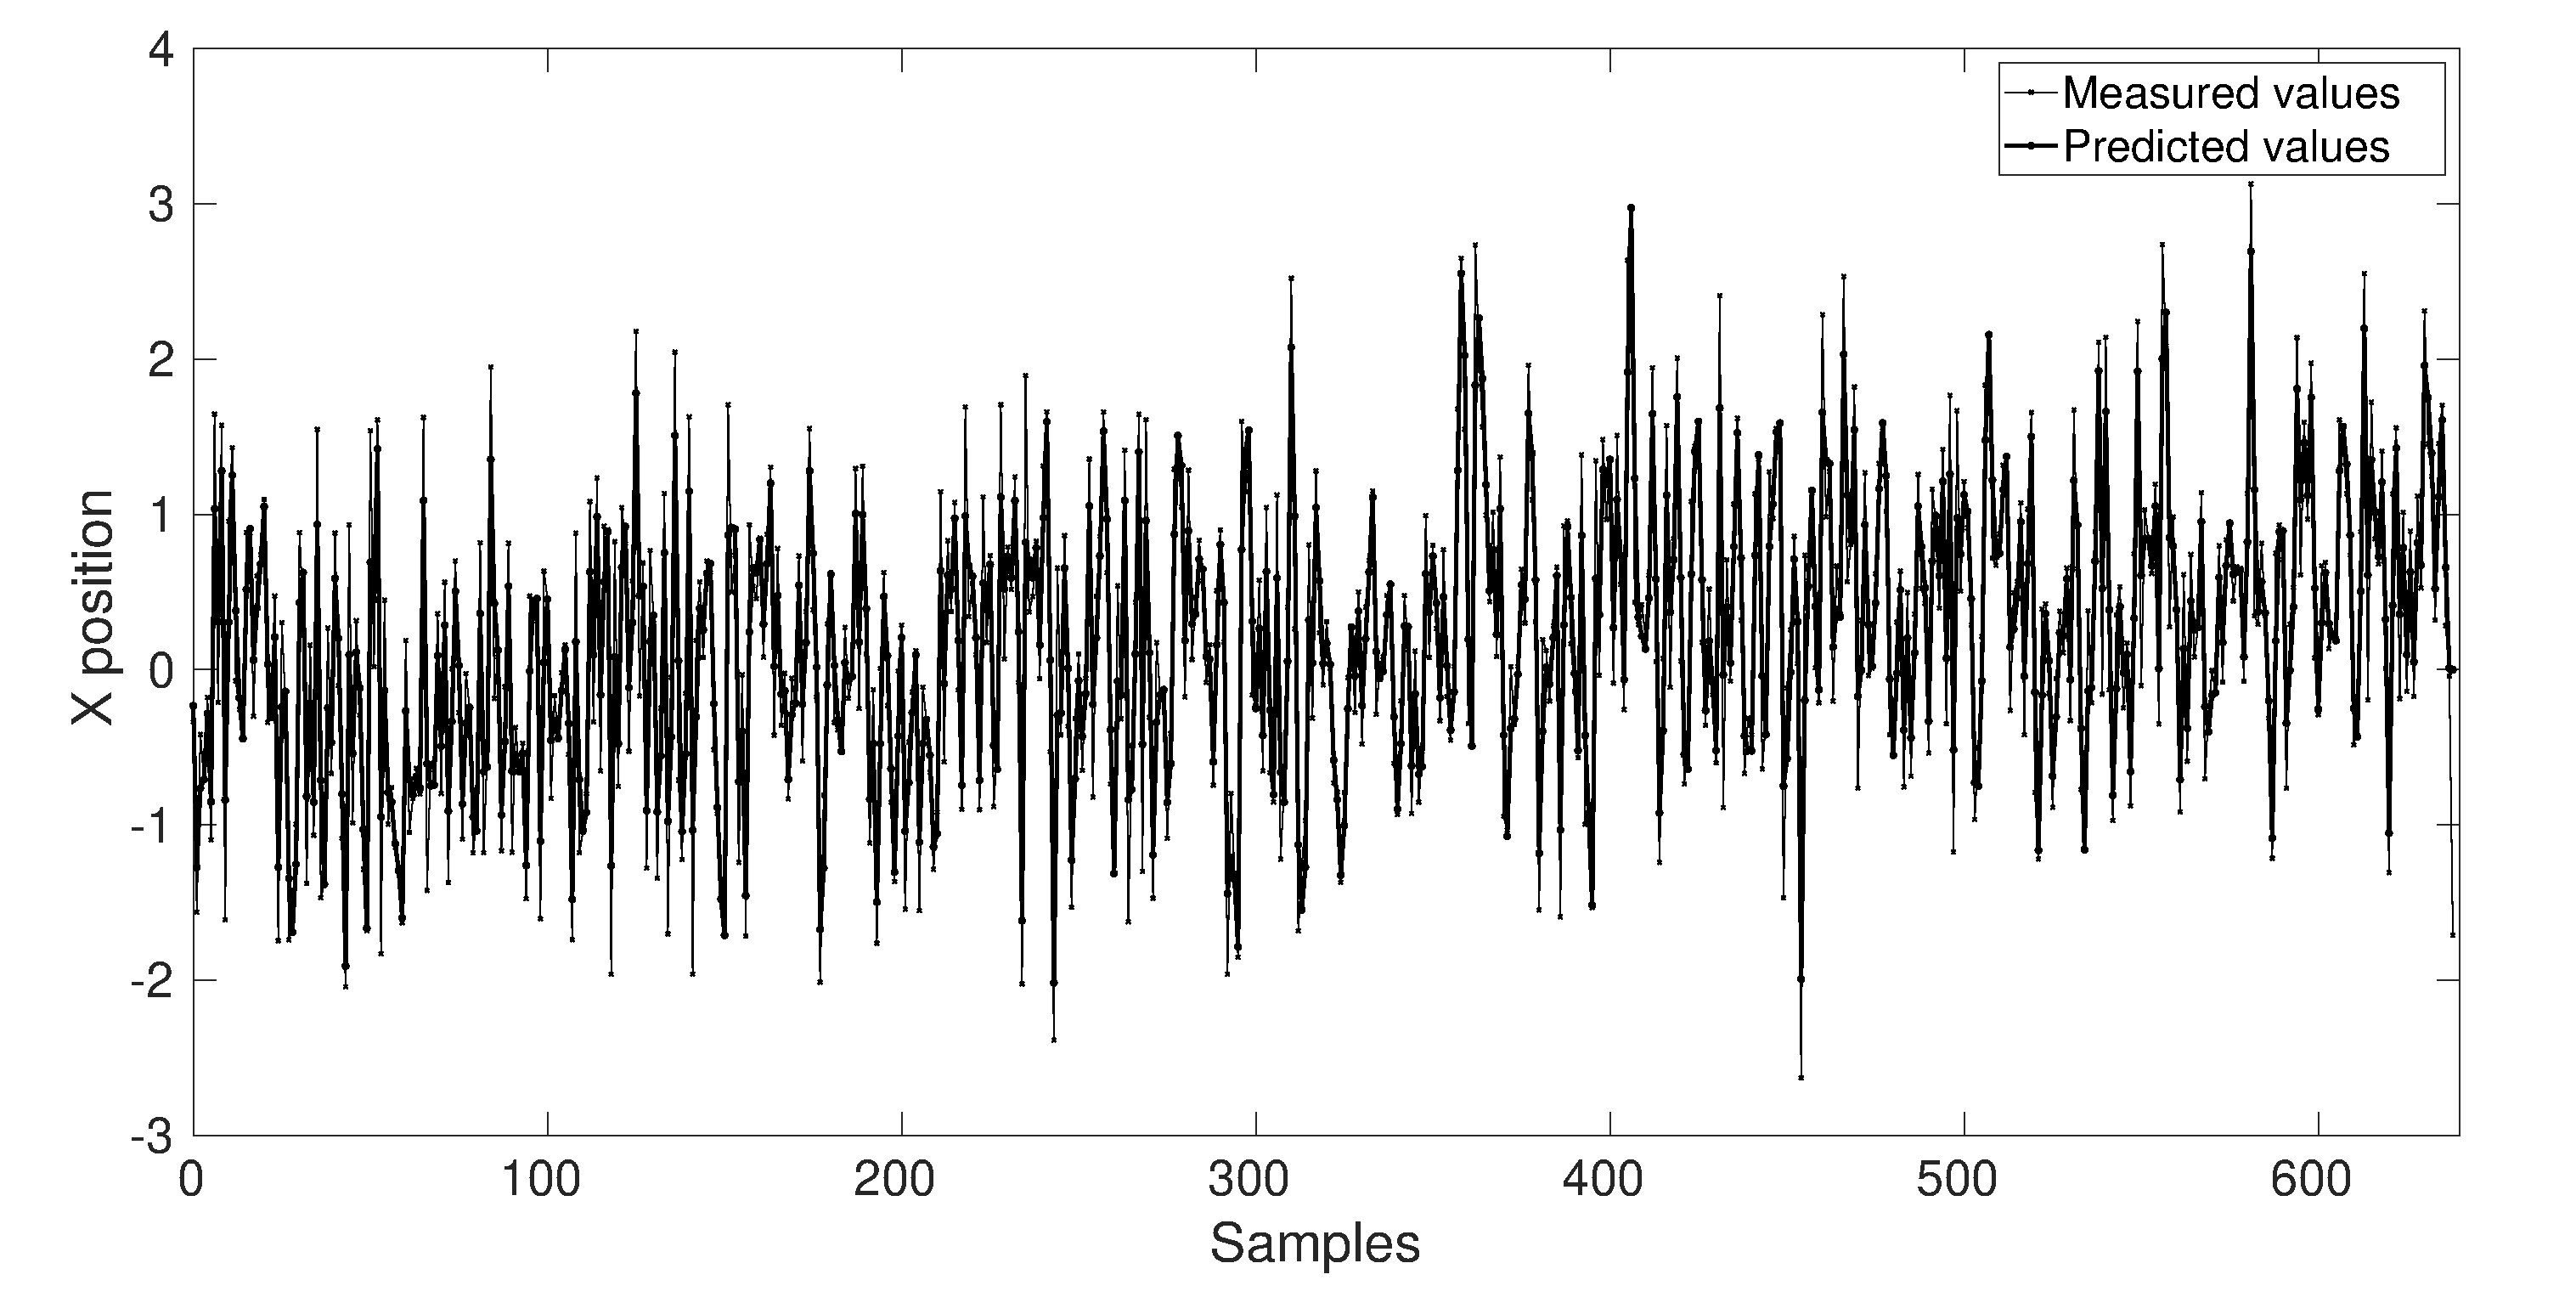
\includegraphics[width = \textwidth]{./Figures/part1Ratio1.eps}
	\caption{Kalman 1D plot for Ratio 1}
	\label{fig:kalman 1D Rat1}
\end{minipage}%
\begin{minipage}{0.5\textwidth}
\centering
	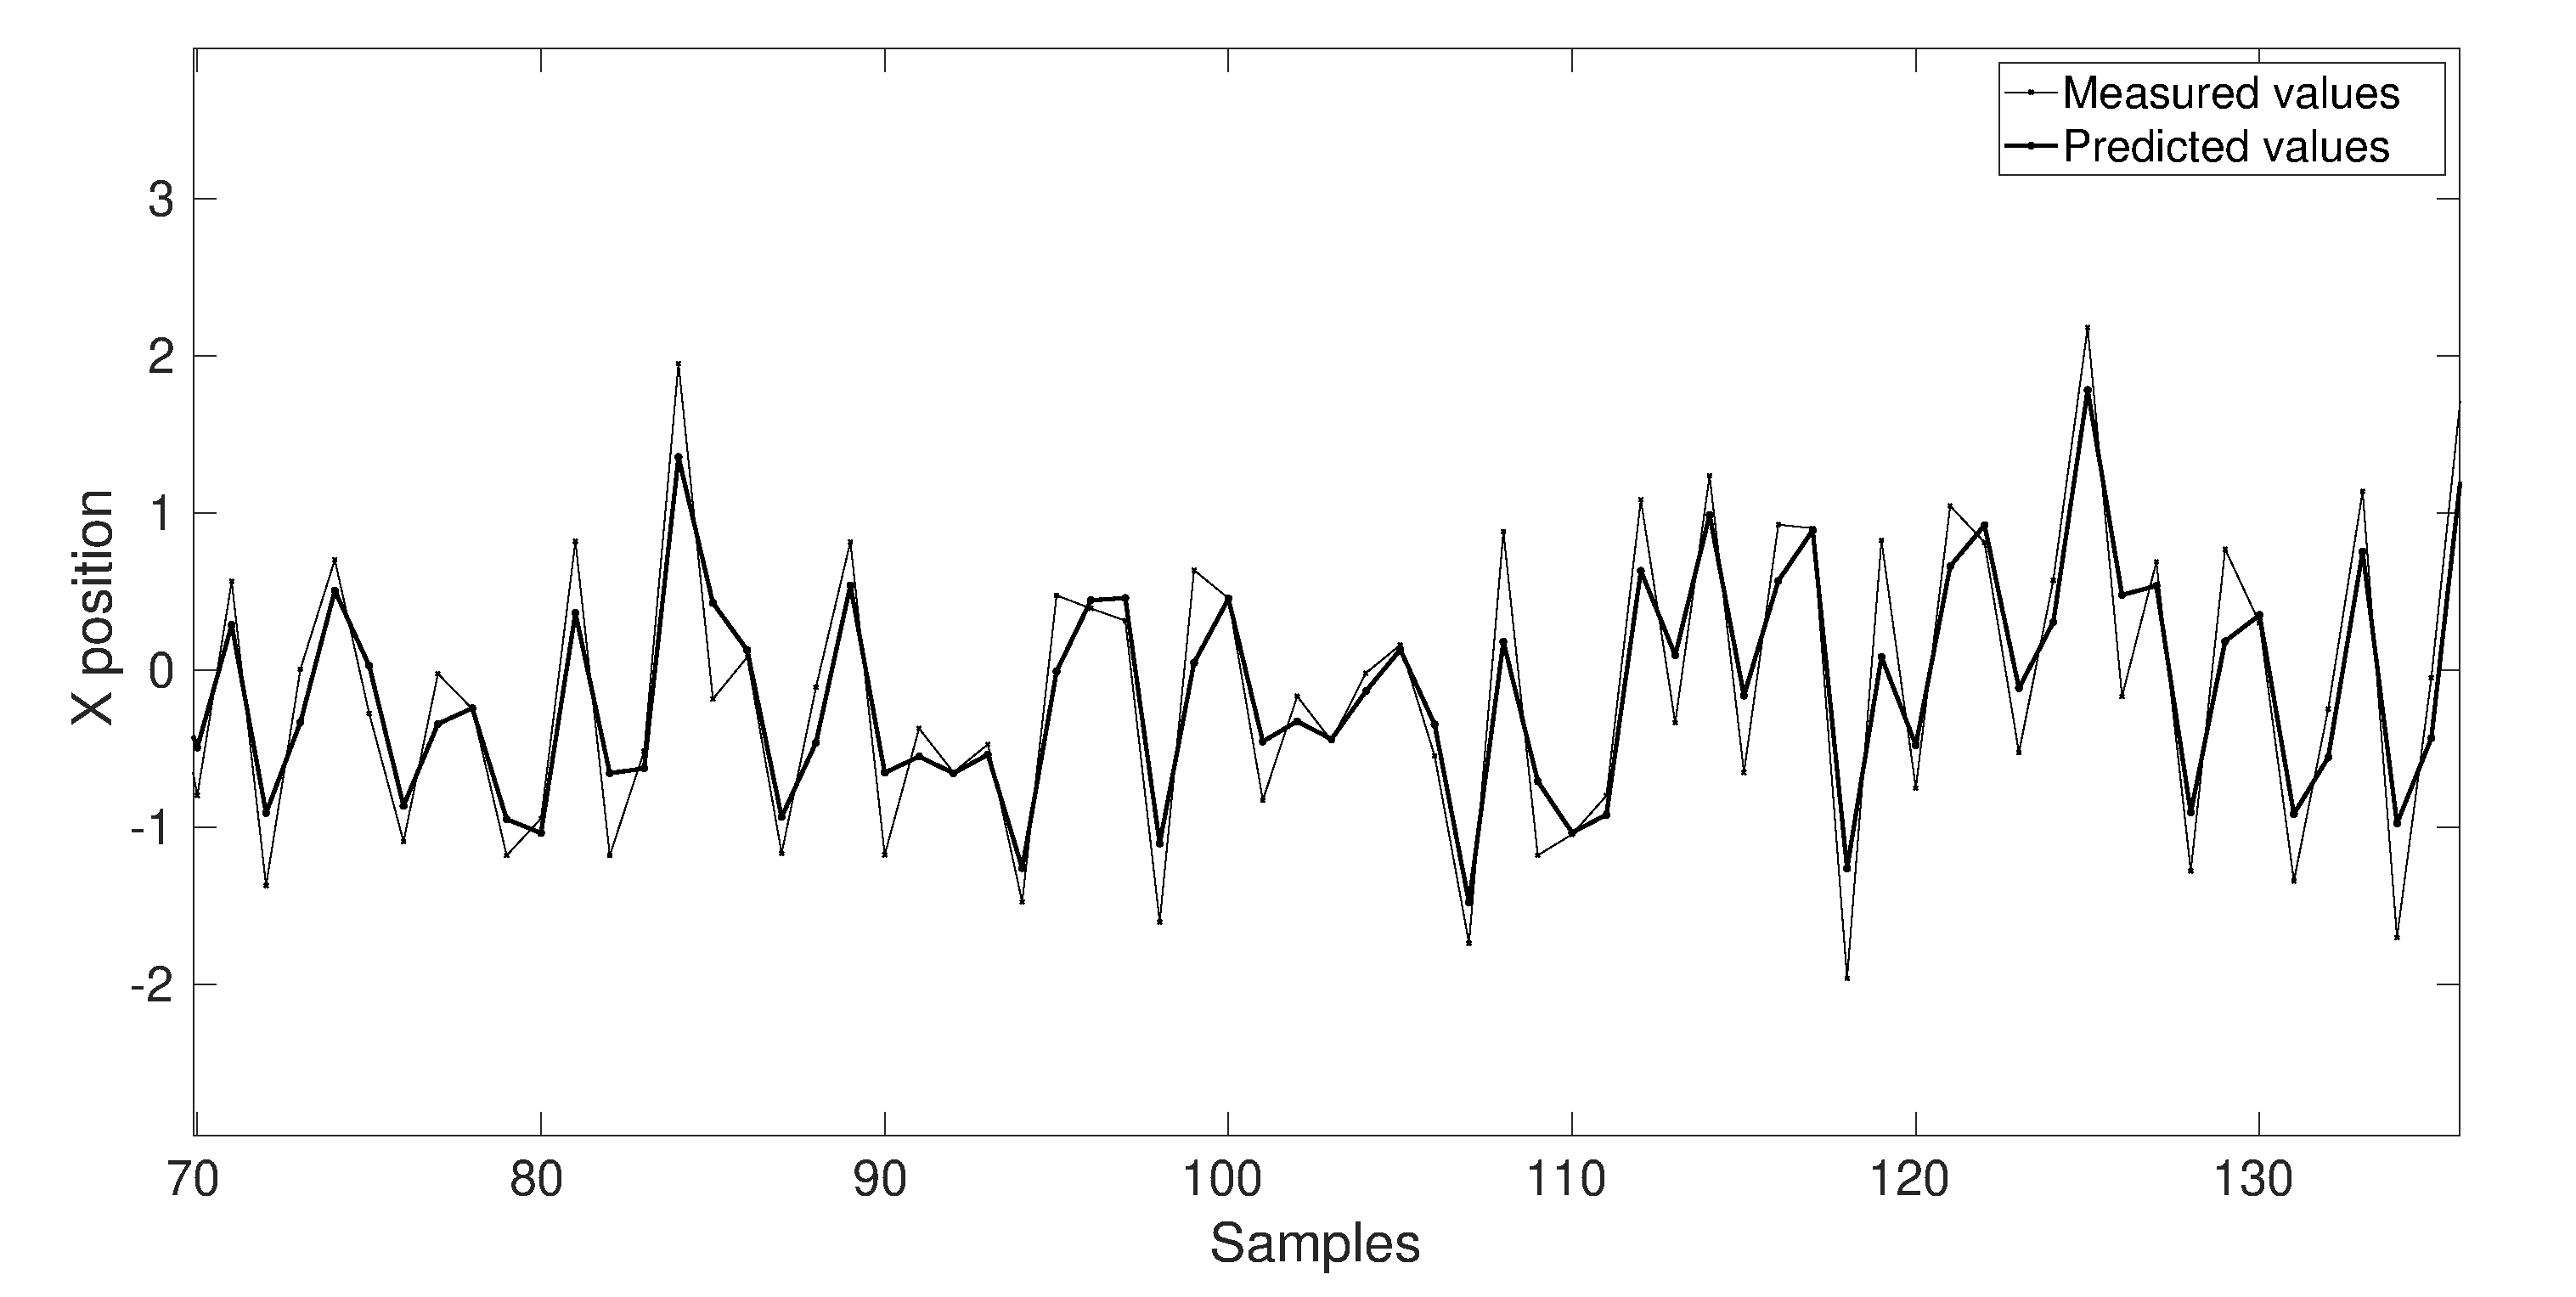
\includegraphics[width = \textwidth]{./Figures/part1Ratio1zoomed.eps}
	\caption{ Zoomed Kalman 1D plot for Ratio 1}
	\label{fig: kalman 1D Rat1 zoom}
\end{minipage}
\end{figure}
\noindent
Figure \ref{fig:kalman 1D Rat1} represents the X-position plot of the given data and the Kalman filter prediction for Ratio 1. Figure \ref{fig: kalman 1D Rat1 zoom} represents the zoomed version of the same plot.\\
For this plot Ratio 1 i.e. \textbf{Measurement noise(R) = 1} and \textbf{dynamic noise(Q) = 1} is considered.\\

\newpage
%RAtio 2 1:0.0001
\begin{figure}[h]
\centering
\begin{minipage}{0.5\textwidth}
\centering
	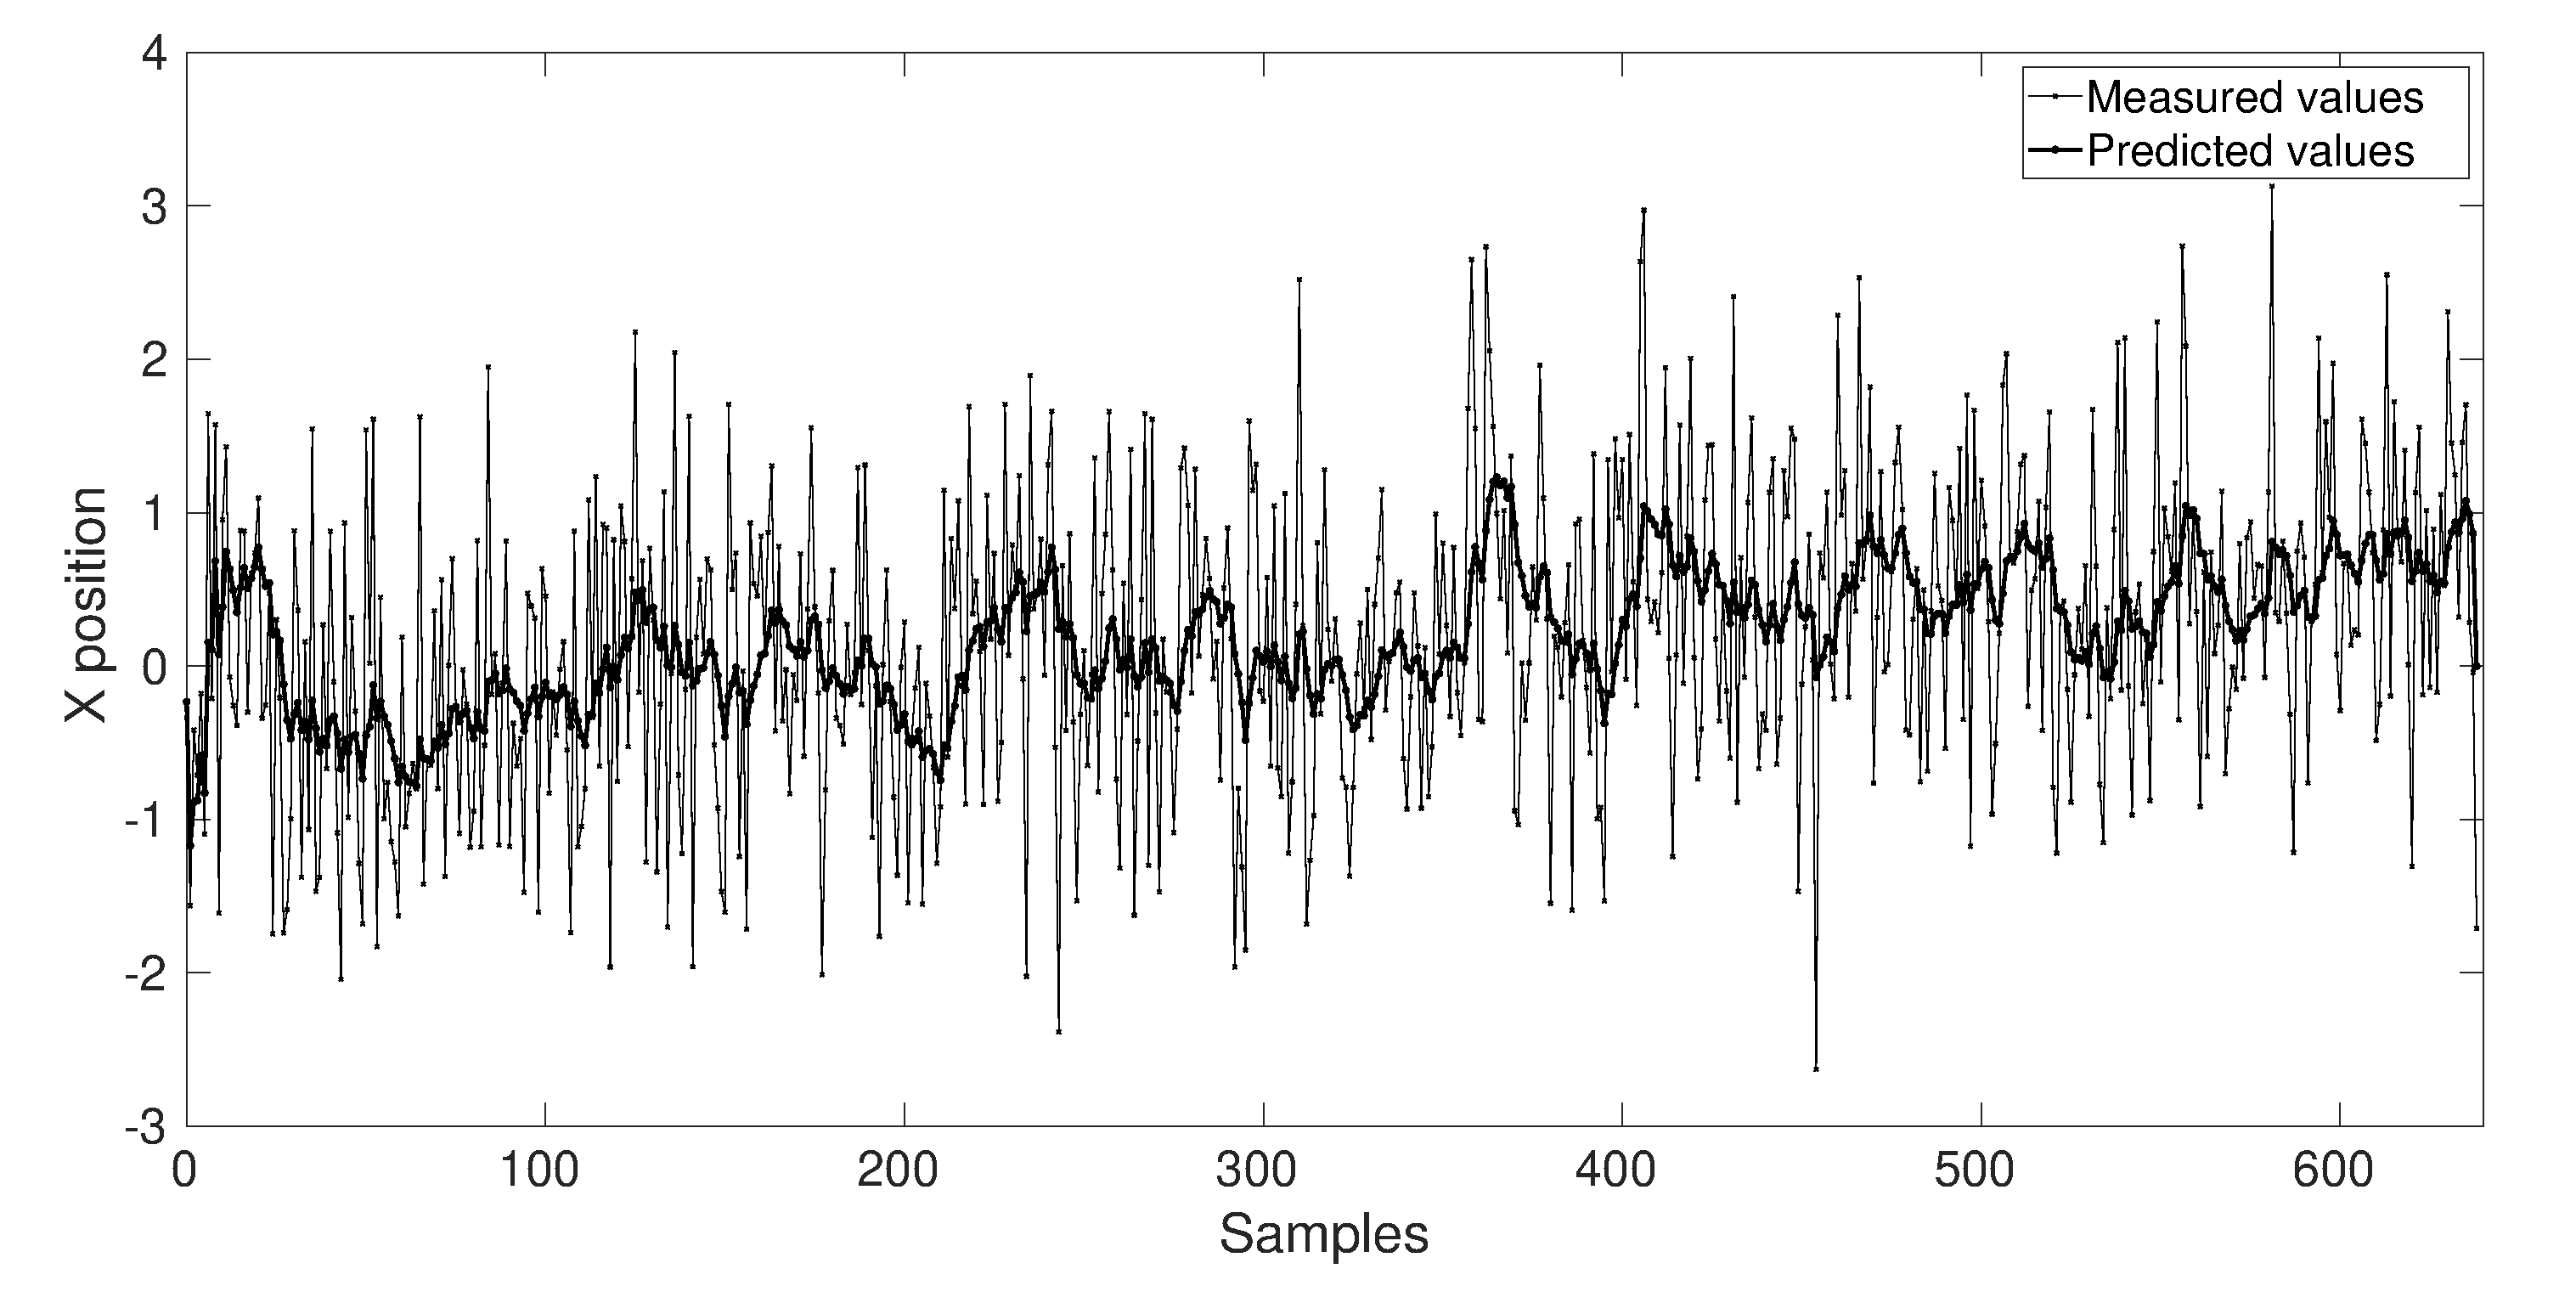
\includegraphics[width = \textwidth]{./Figures/part1Ratio2.eps}
	\caption{Kalman 1D plot for Ratio 2}
	\label{fig:kalman 1D Rat2}
\end{minipage}%
\begin{minipage}{0.5\textwidth}
\centering
	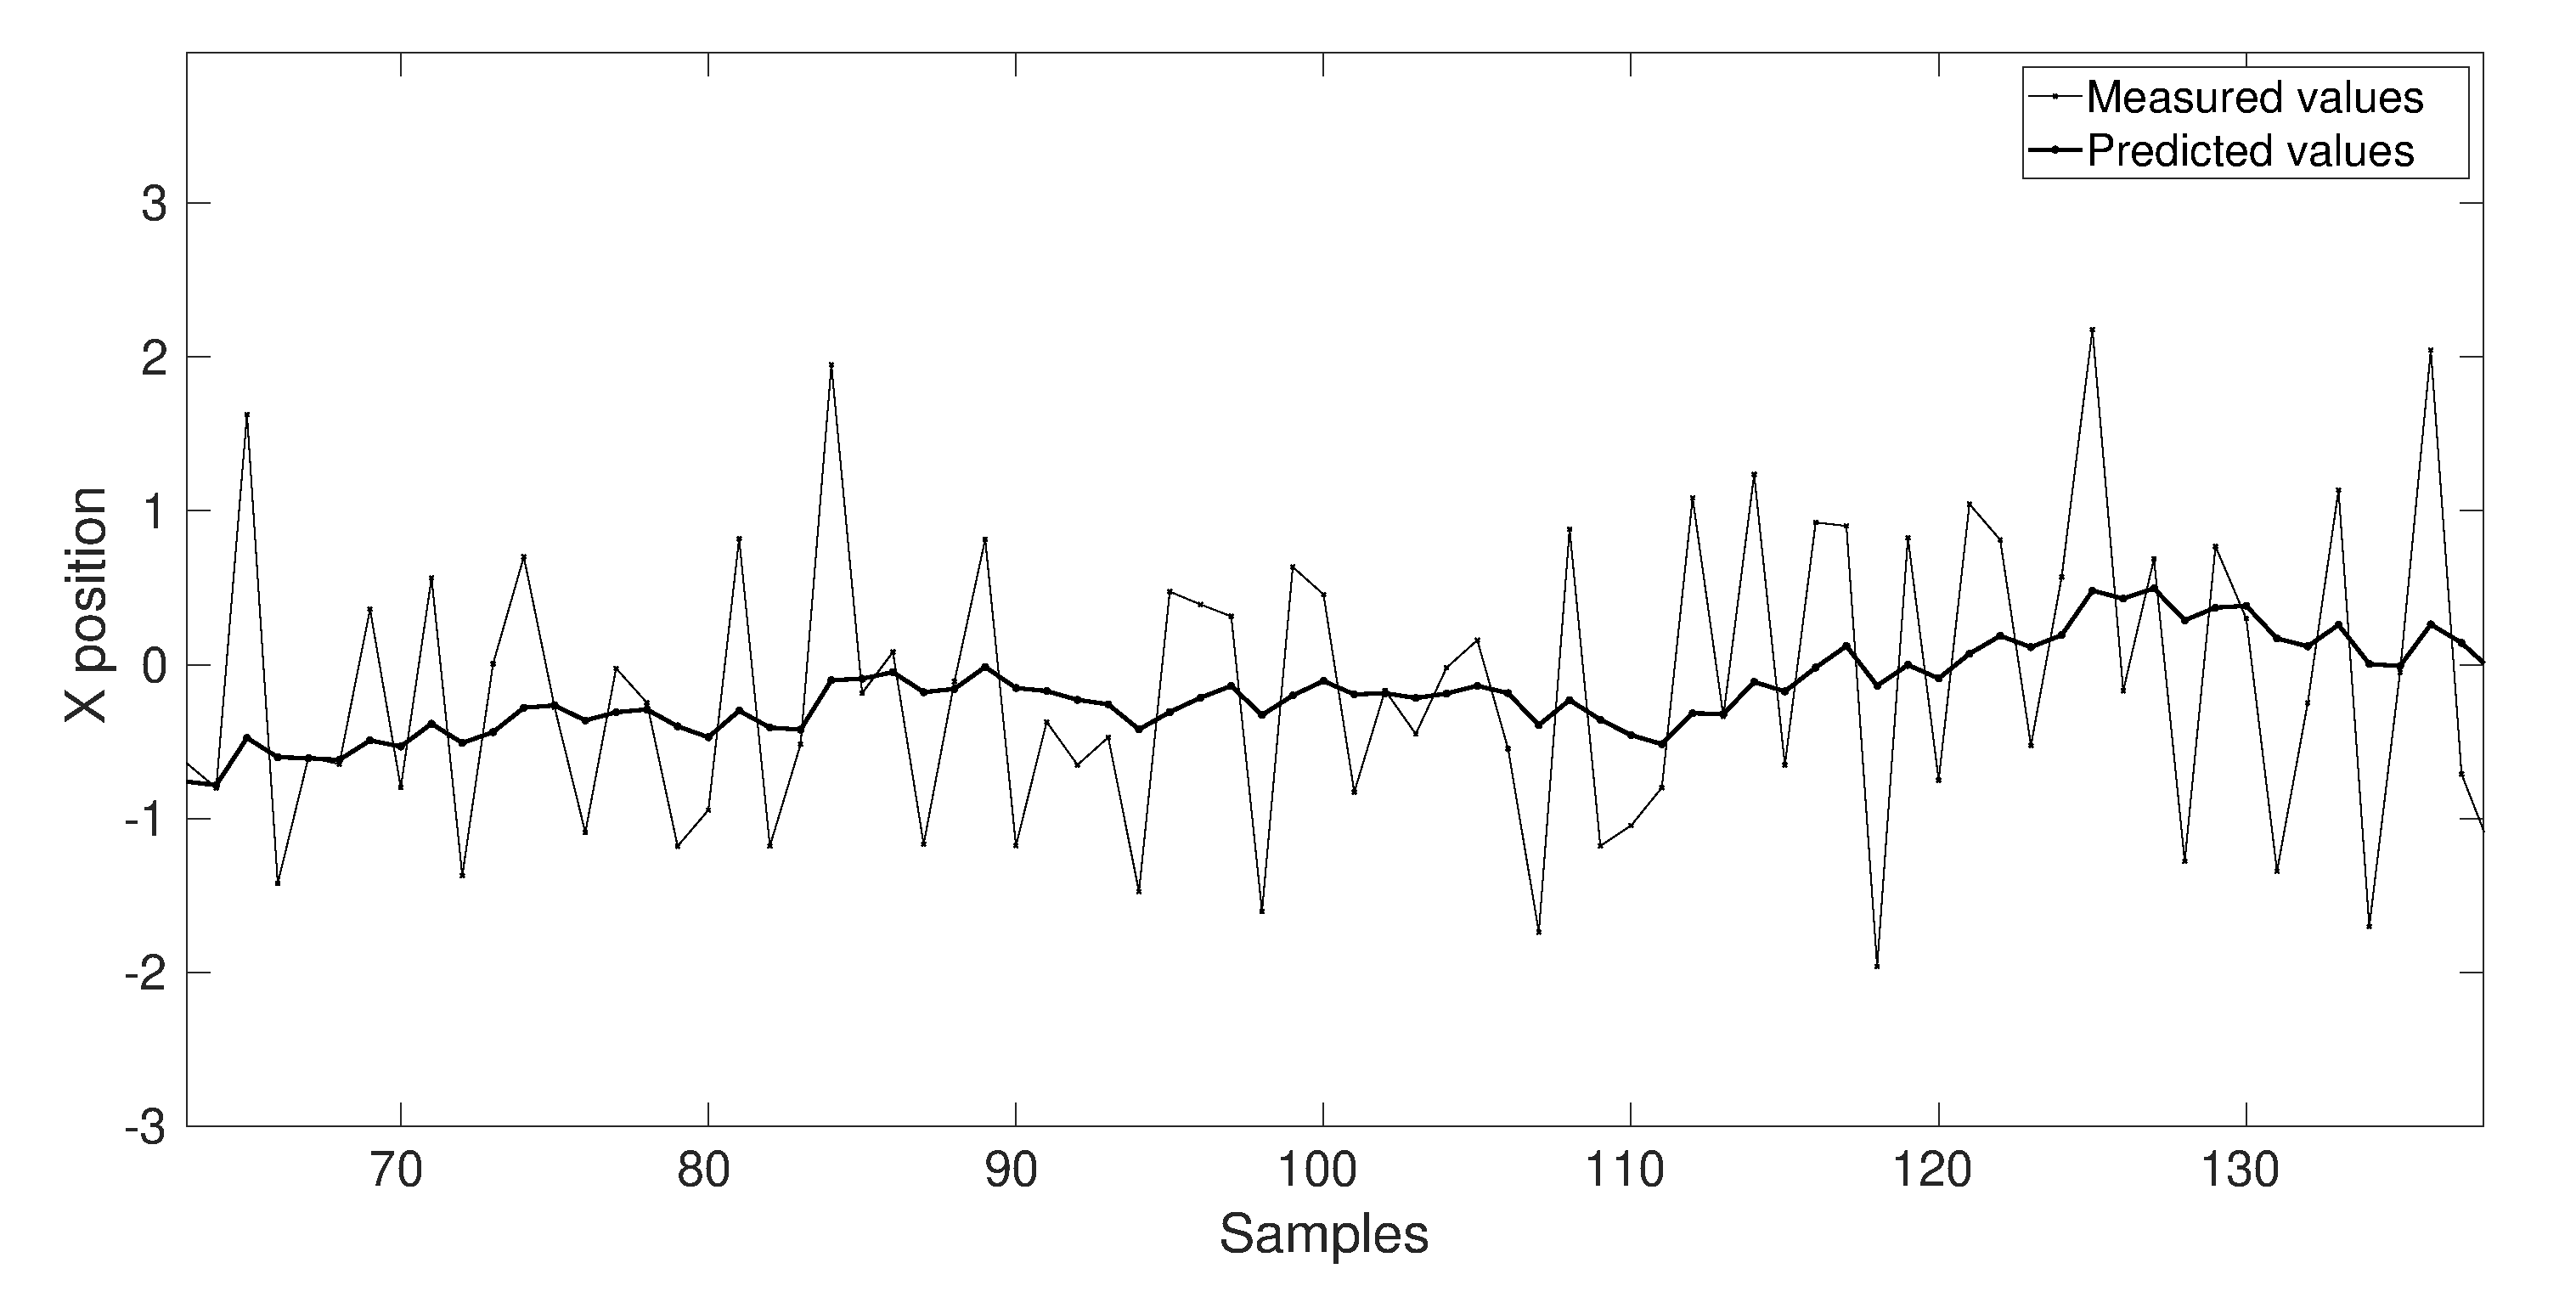
\includegraphics[width = \textwidth]{./Figures/part1Ratio2zoomed.eps}
	\caption{ Zoomed Kalman 1D plot for Ratio 2}
	\label{fig: kalman 1D Rat2 zoom}
\end{minipage}
\end{figure}
\noindent
Figure \ref{fig:kalman 1D Rat2} represents the X-position plot of the given data and the Kalman filter prediction for Ratio 2. Figure \ref{fig: kalman 1D Rat2 zoom} represents the zoomed version of the same plot.\\
For this plot Ratio 2 i.e. \textbf{Measurement noise(R) = 1} and \textbf{dynamic noise(Q) = 0.0001} is considered.\\

%RAtio 3 1:0.000001
\begin{figure}[h]
\centering
\begin{minipage}{0.5\textwidth}
\centering
	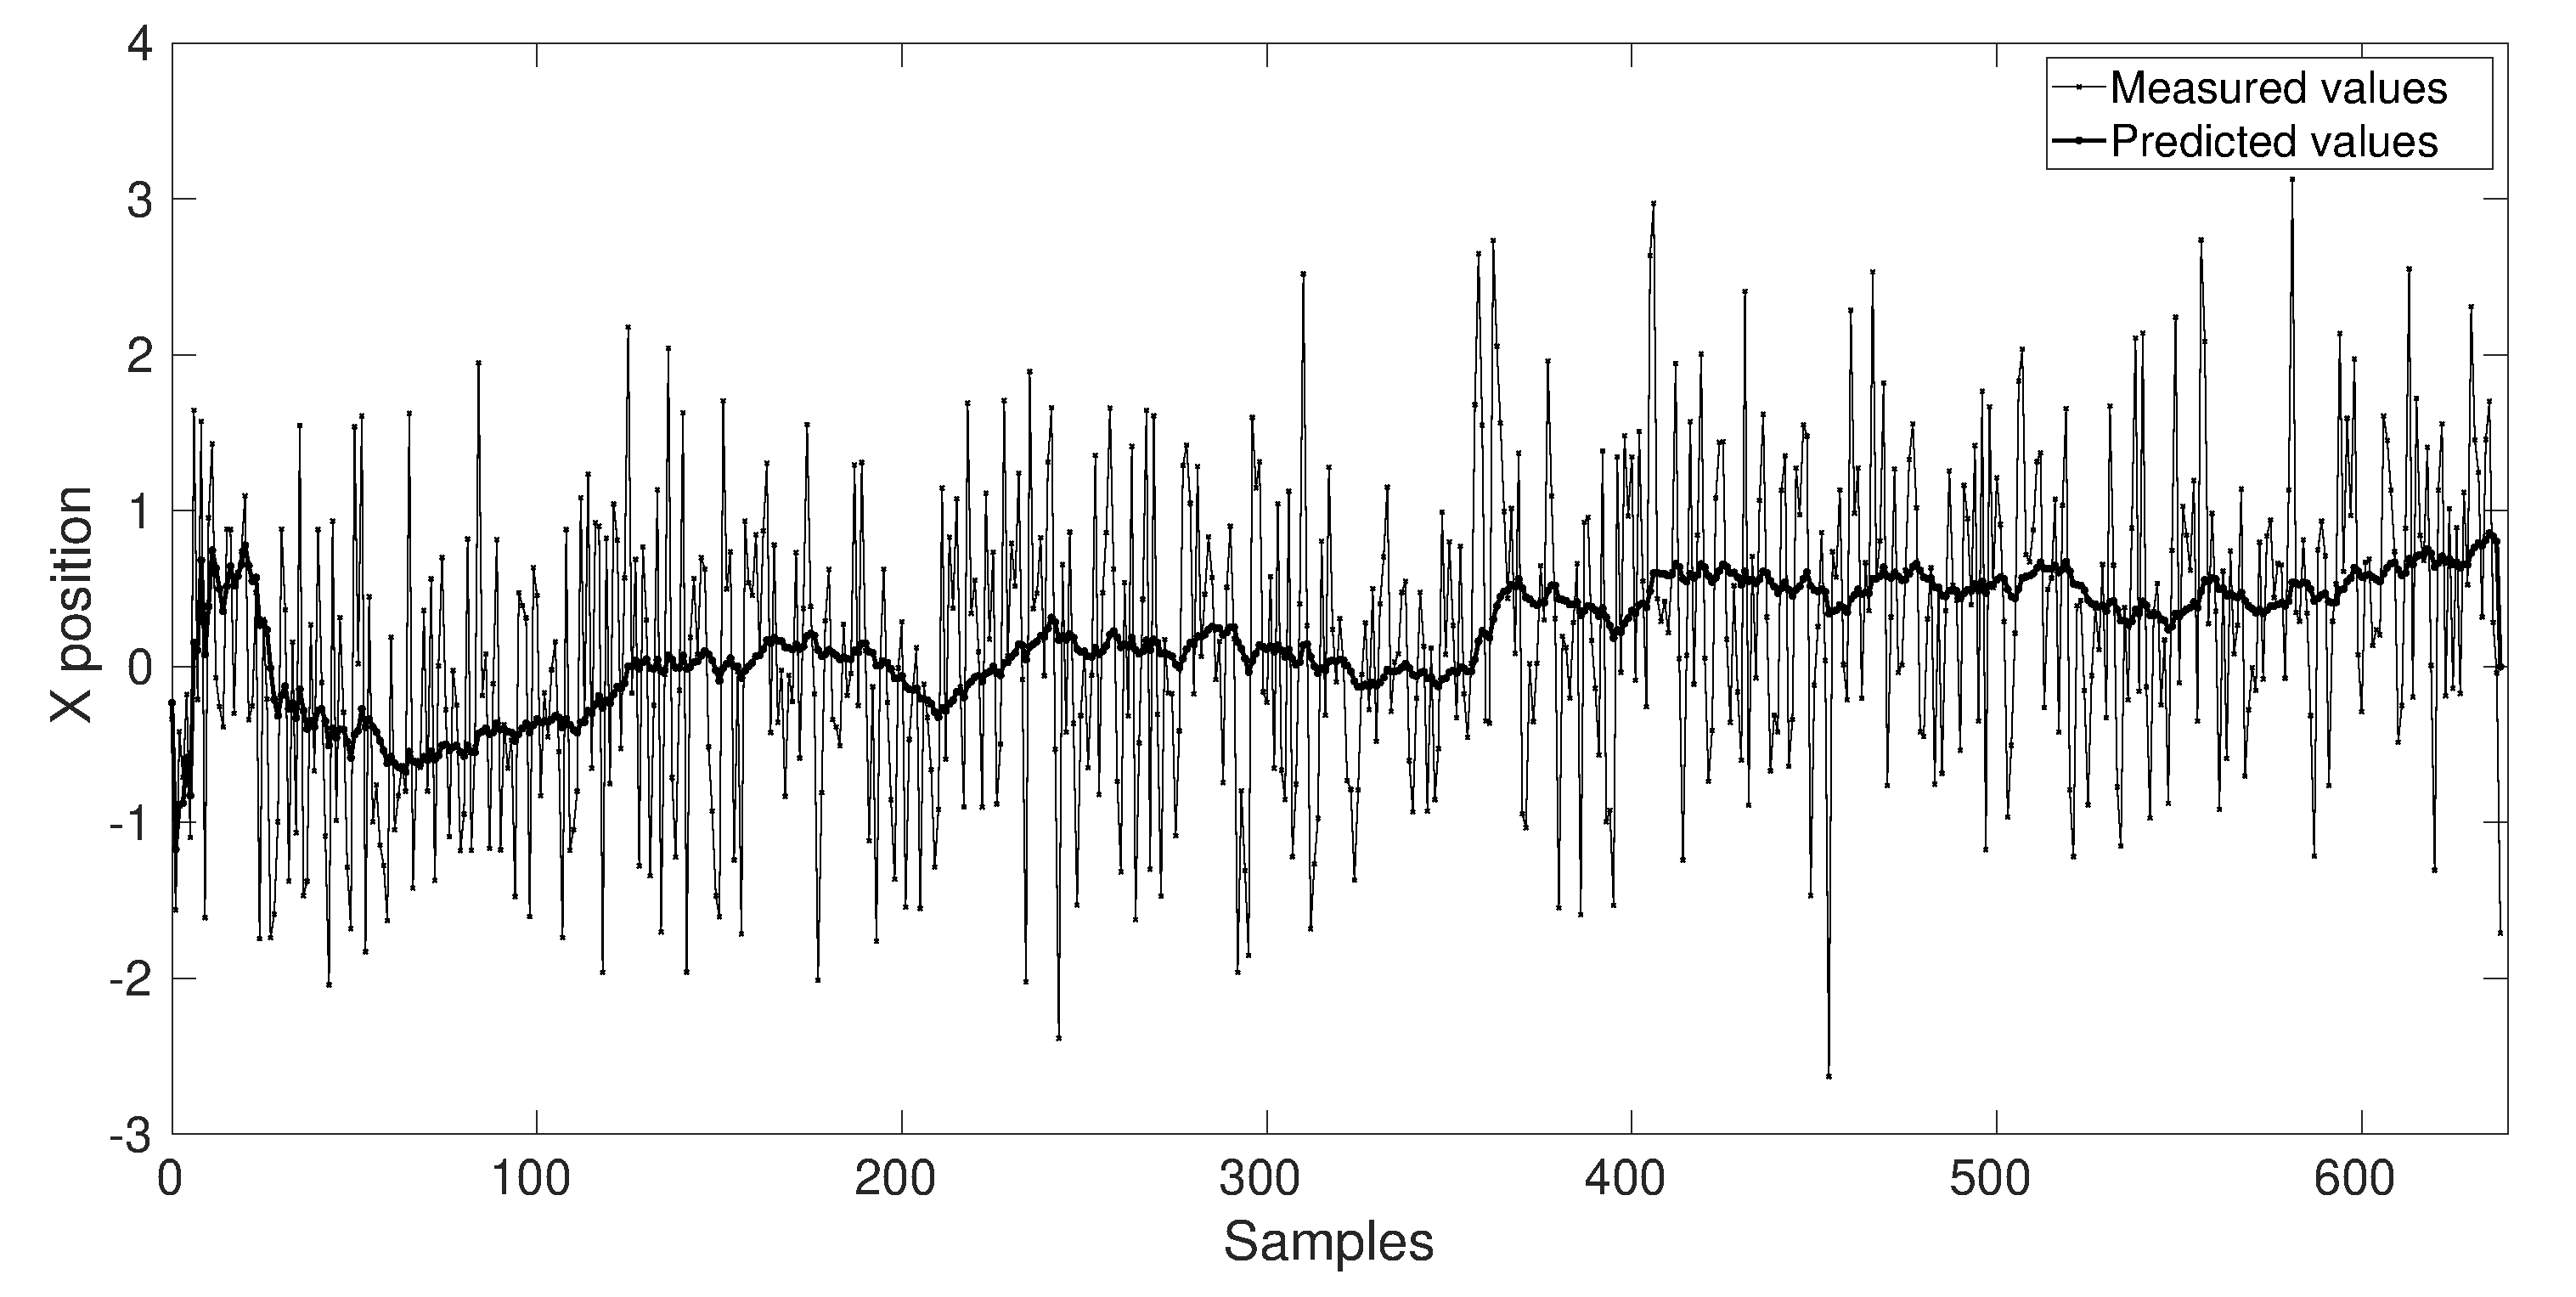
\includegraphics[width = \textwidth]{./Figures/part1Ratio3.eps}
	\caption{Kalman 1D plot for Ratio 3}
	\label{fig:kalman 1D Rat3}
\end{minipage}%
\begin{minipage}{0.5\textwidth}
\centering
	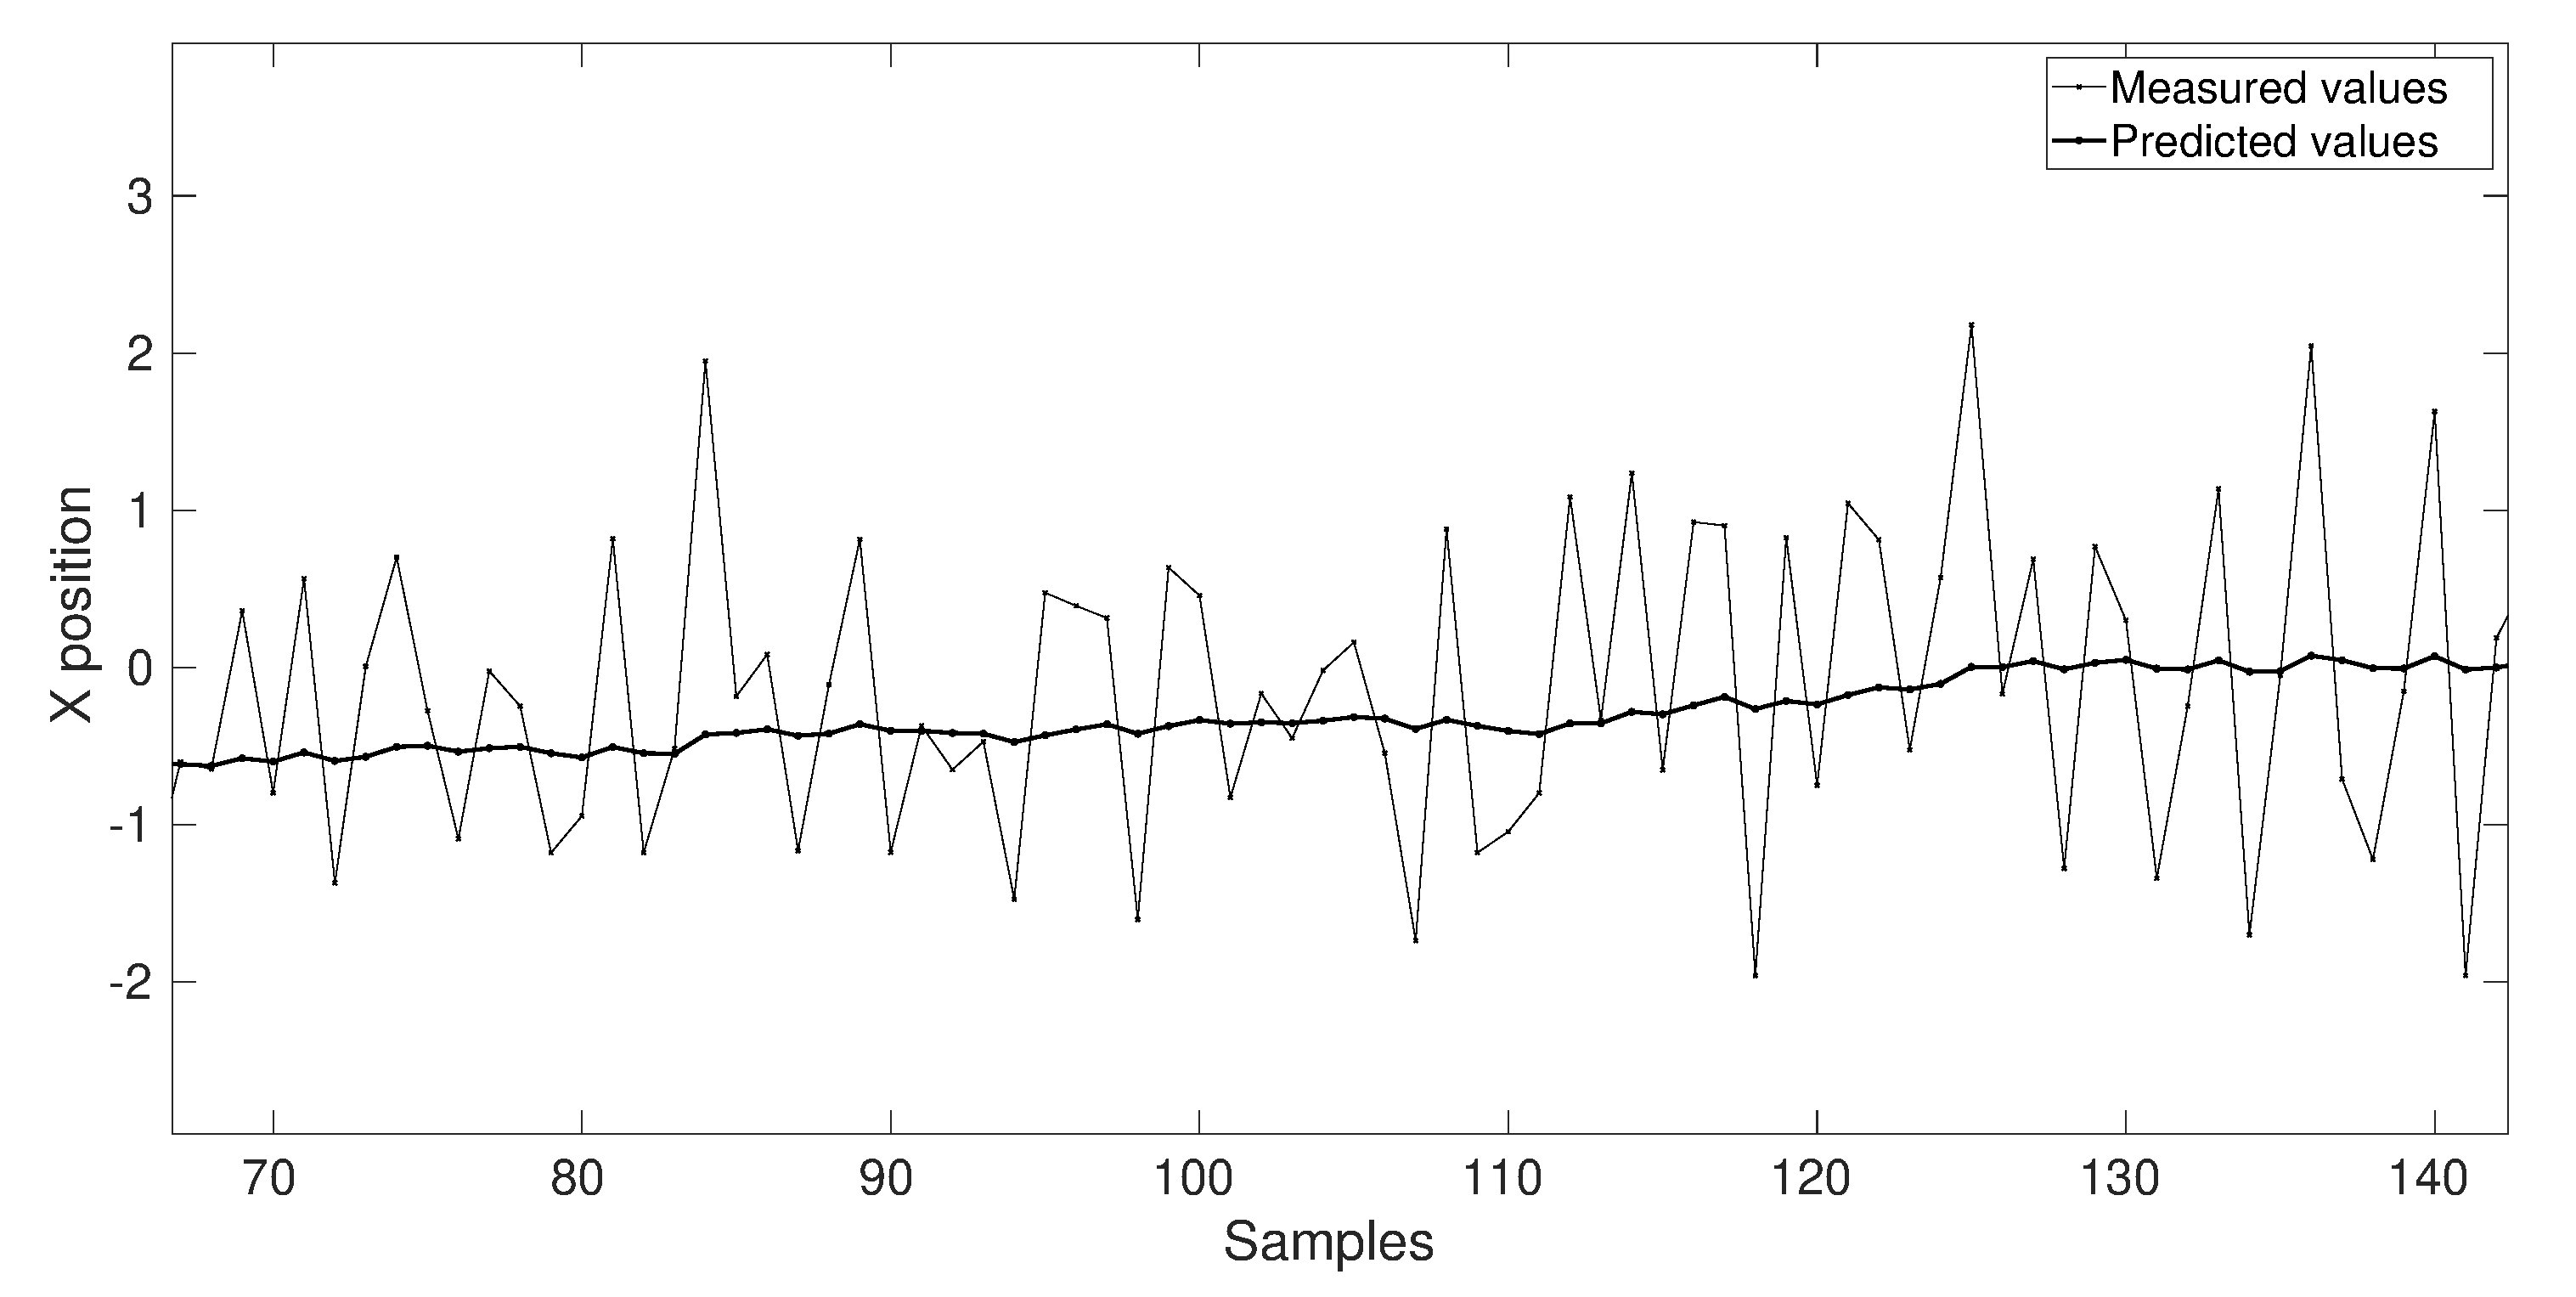
\includegraphics[width = \textwidth]{./Figures/part1Ratio3zoomed.eps}
	\caption{ Zoomed Kalman 1D plot for Ratio 3}
	\label{fig: kalman 1D Rat3 zoom}
\end{minipage}
\end{figure}
\noindent
Figure \ref{fig:kalman 1D Rat3} represents the X-position plot of the given data and the Kalman filter prediction for Ratio 2. Figure \ref{fig: kalman 1D Rat3 zoom} represents the zoomed version of the same plot.\\
For this plot Ratio 3 i.e. \textbf{Measurement noise(R) = 1} and \textbf{dynamic noise(Q) = 0.000001} is considered.\\
\newpage

%----------------------Part2------------------------------------
%RAtio 1 0.1:0.001
\begin{figure}[ht!]
\centering
\begin{minipage}{0.5\textwidth}
\centering
	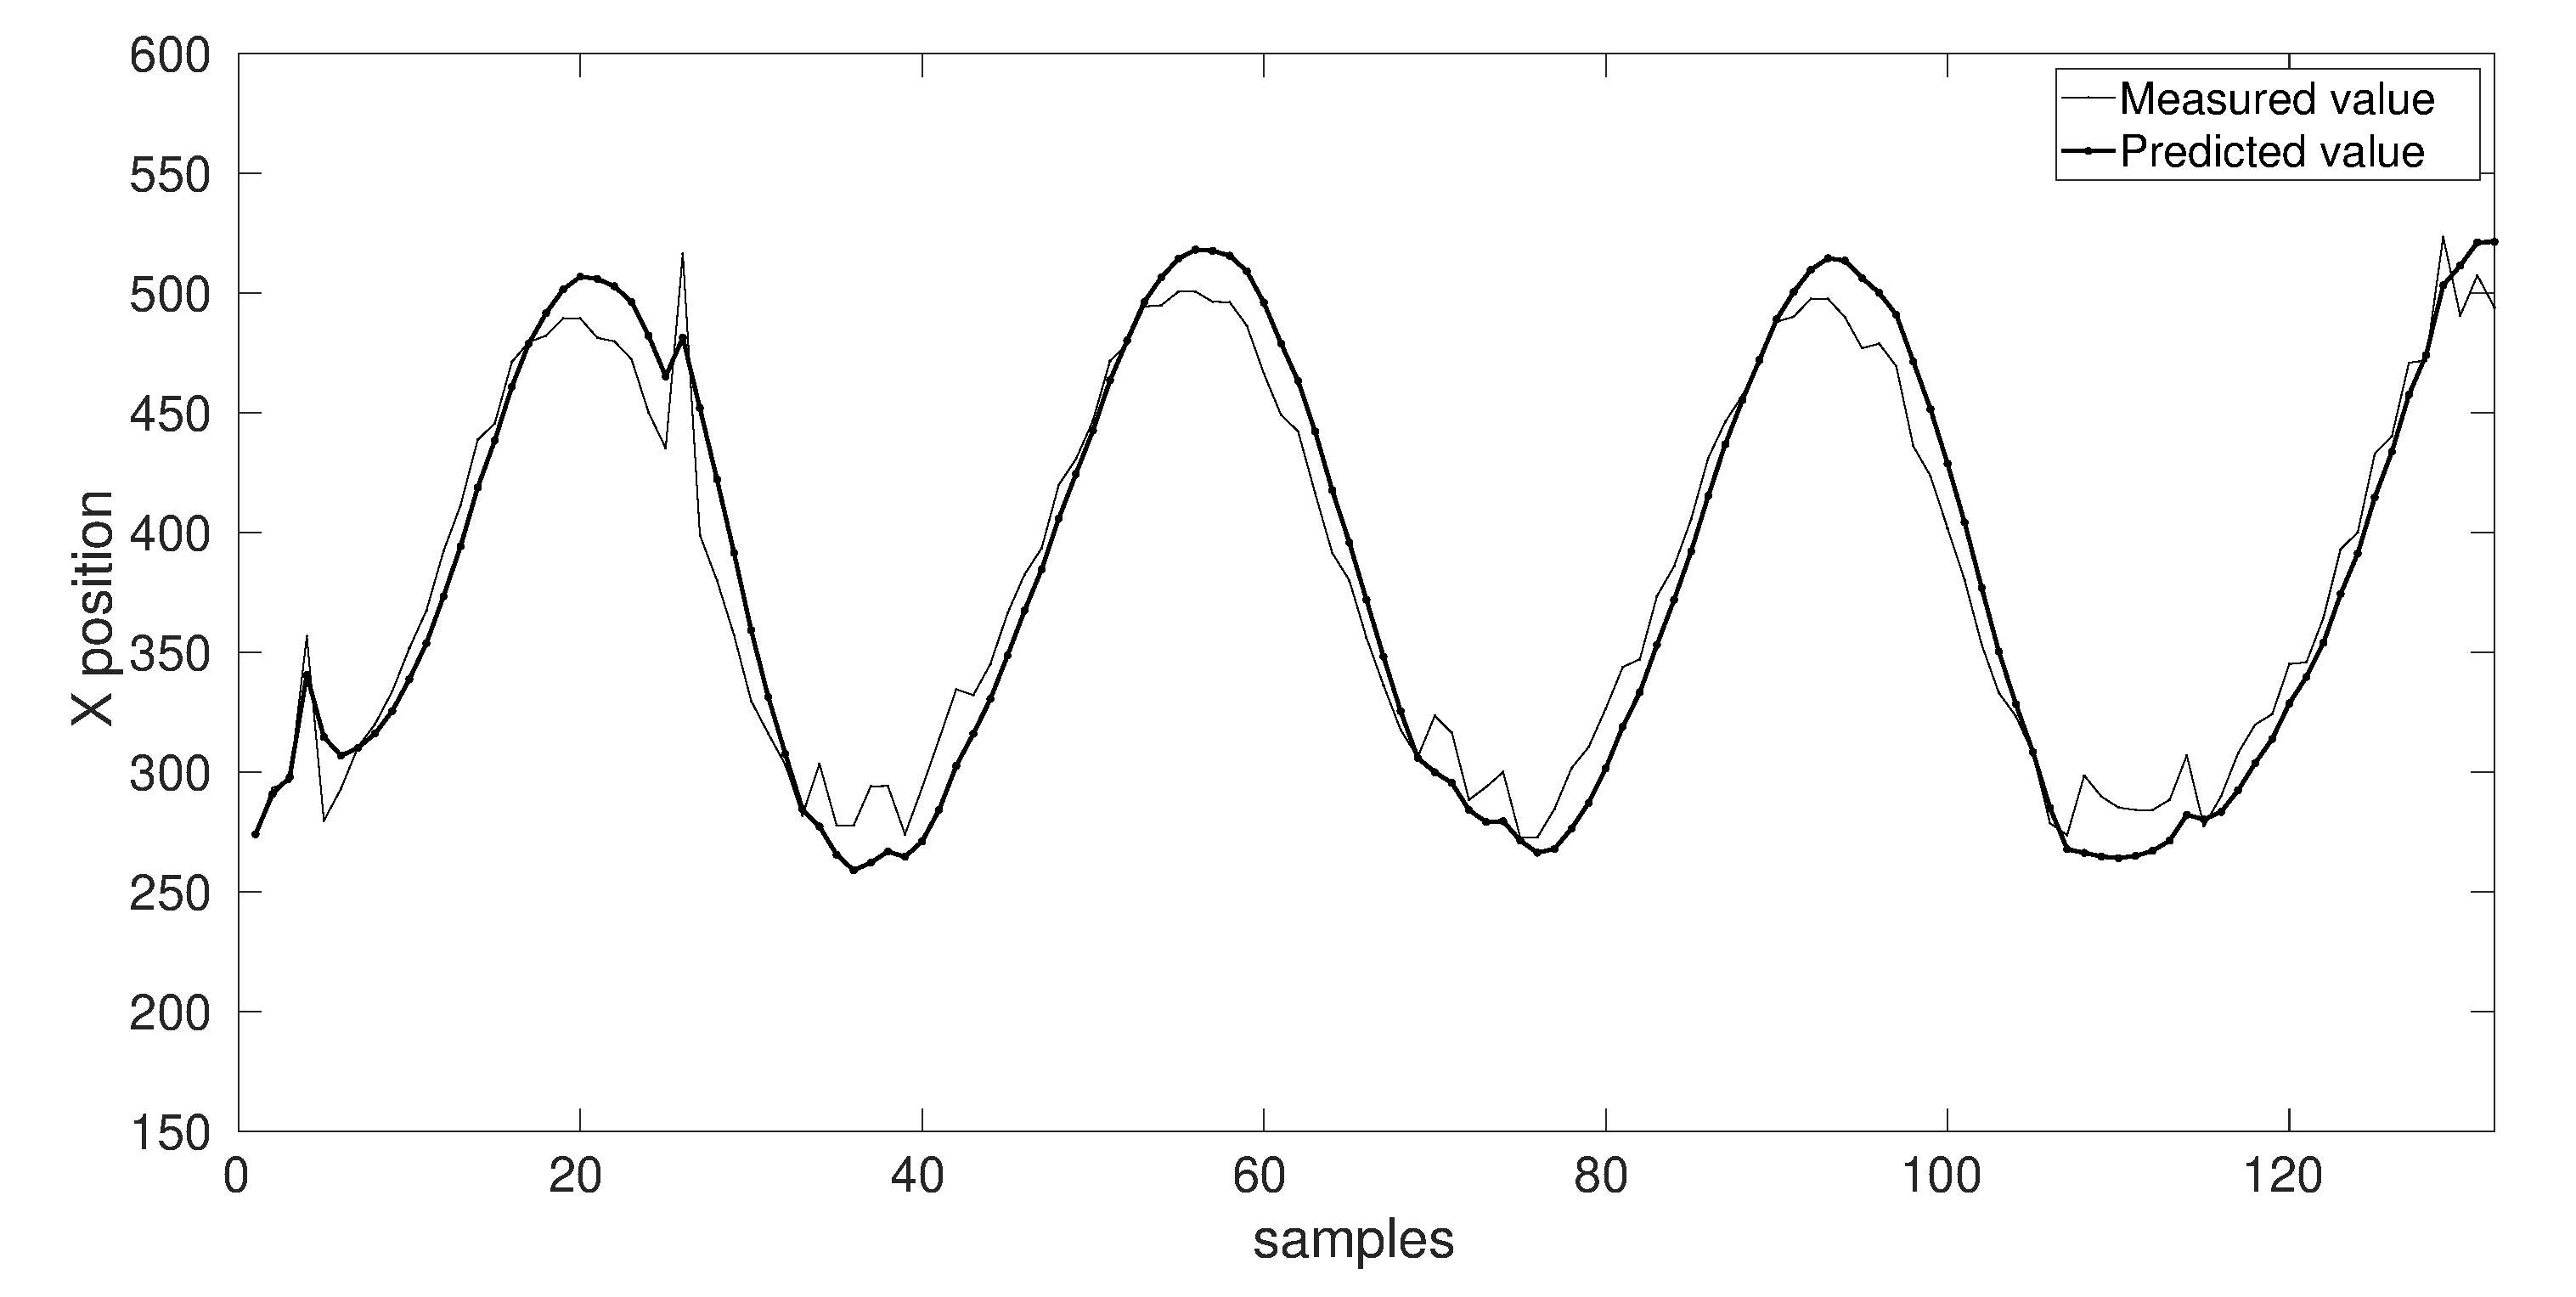
\includegraphics[width = \textwidth]{./Figures/part2Ratio1X.eps}
	\caption{Kalman 2D X-position plot for Ratio 1}
	\label{fig:kalman 2D XRat1}
\end{minipage}%%
\begin{minipage}{0.5\textwidth}
\centering
	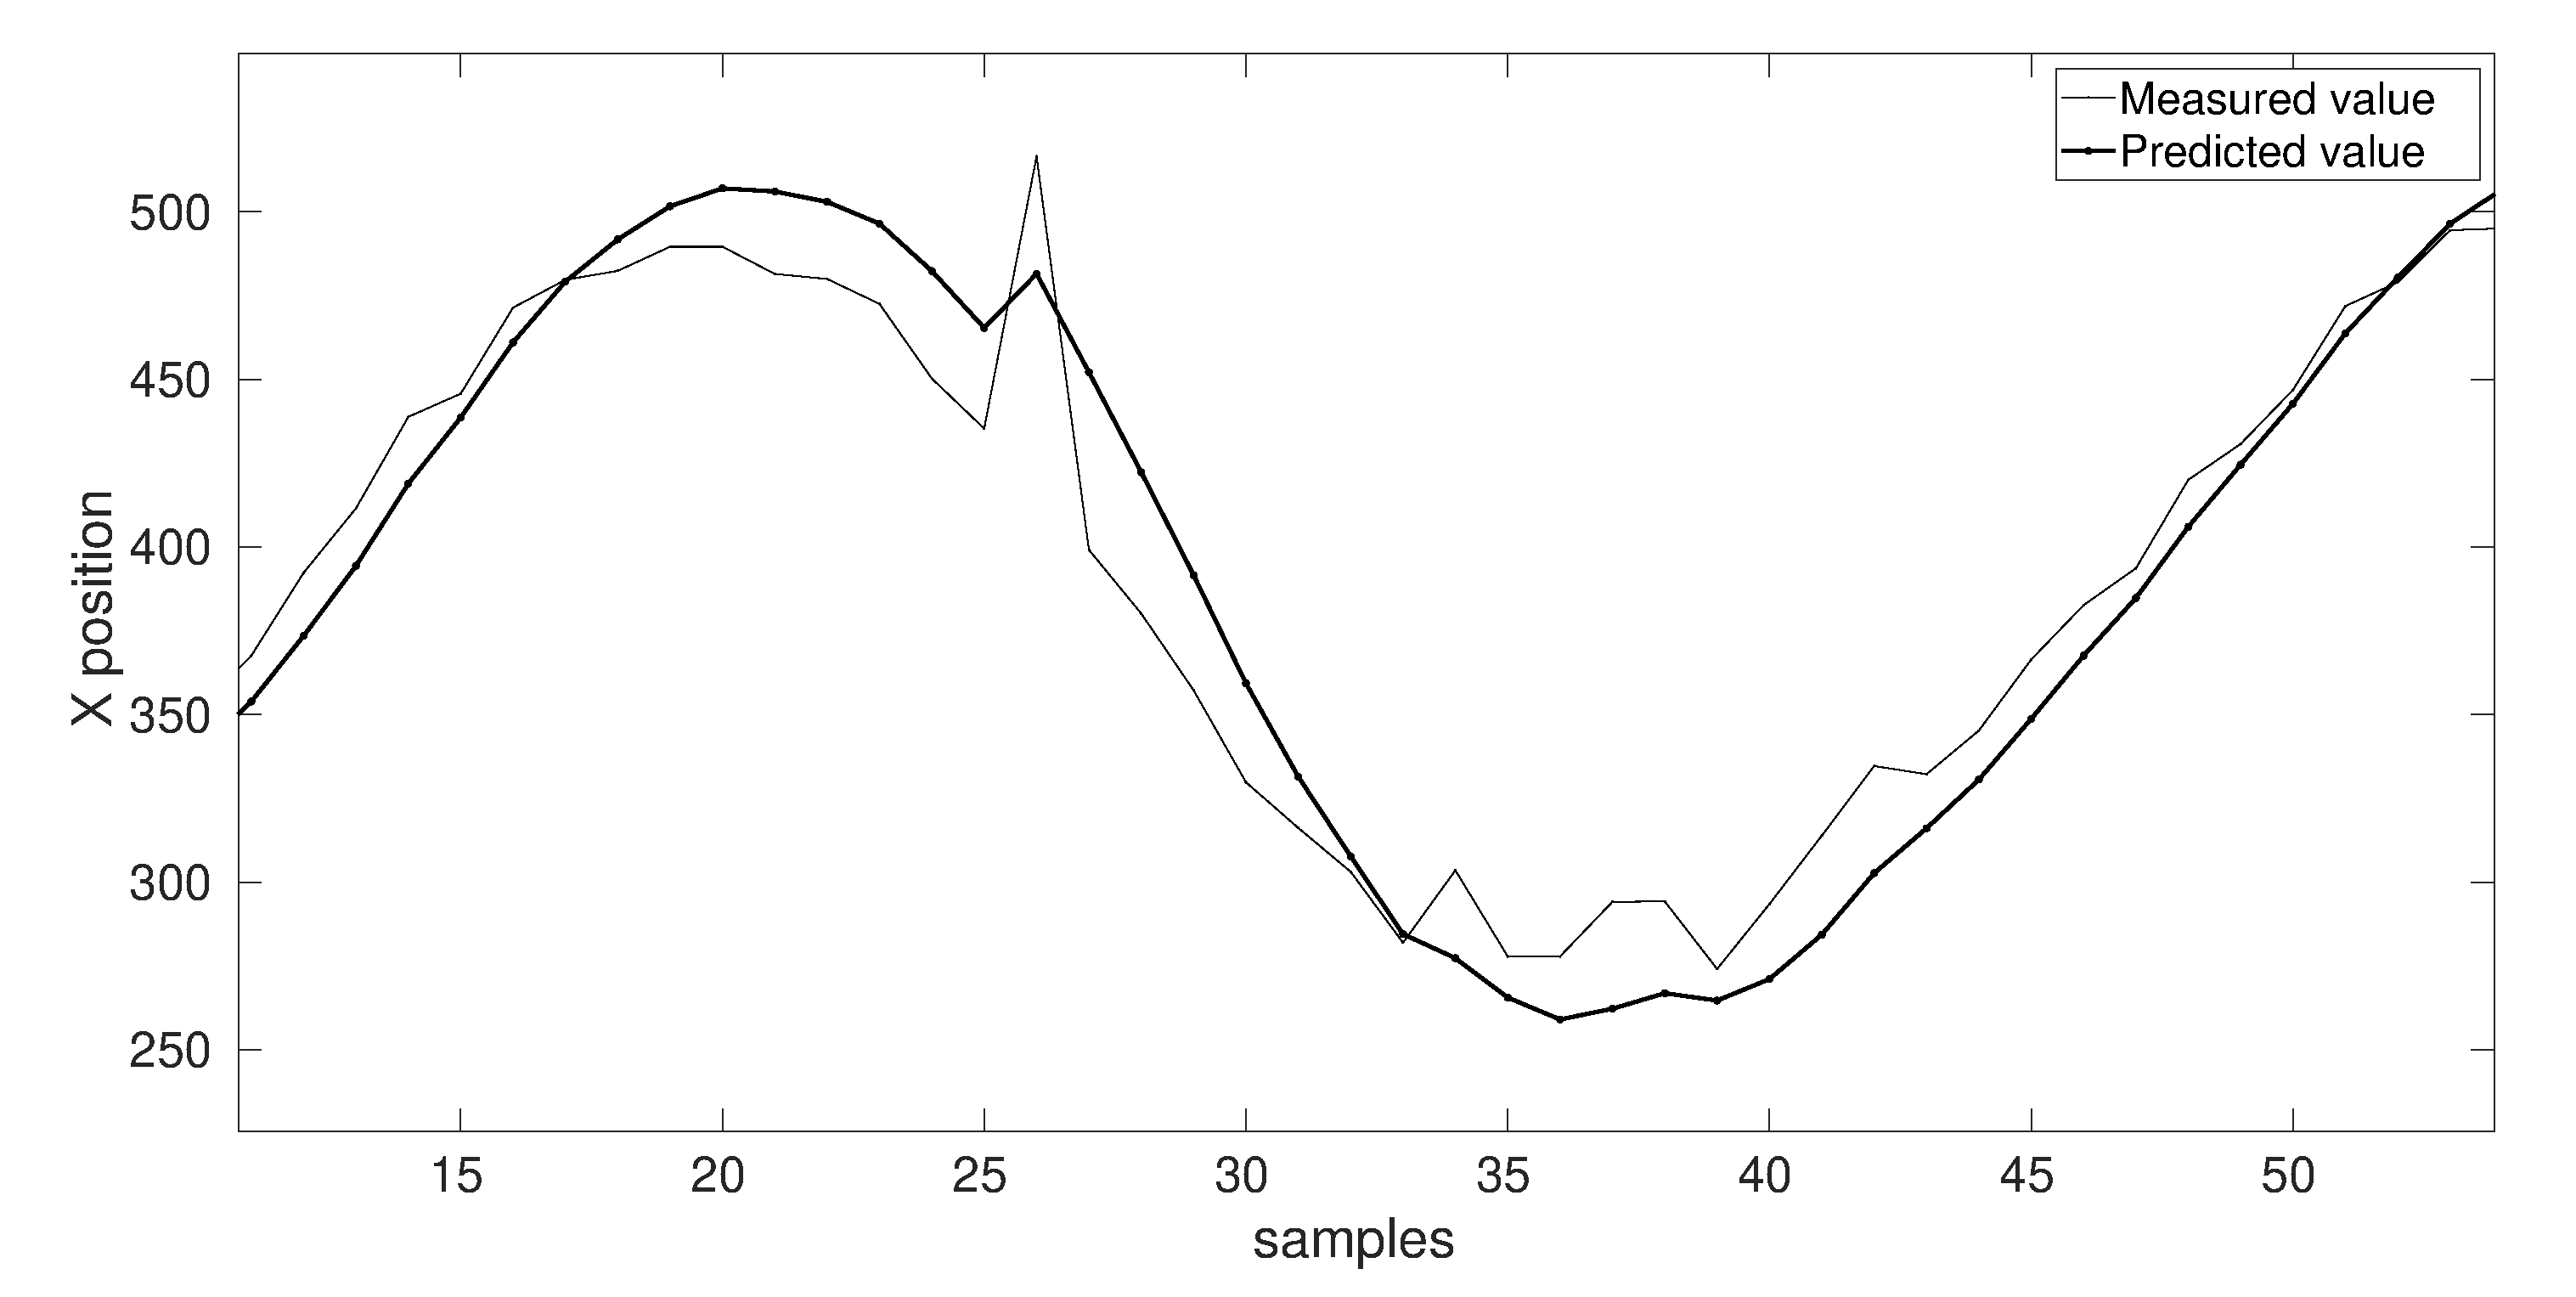
\includegraphics[width = \textwidth]{./Figures/part2Ratio1Xzoomed.eps}
	\caption{ Zoomed X-position plot for Ratio 1}
	\label{fig: kalman 2D XRat1 zoom}
\end{minipage}
\begin{minipage}{0.5\textwidth}
\centering
	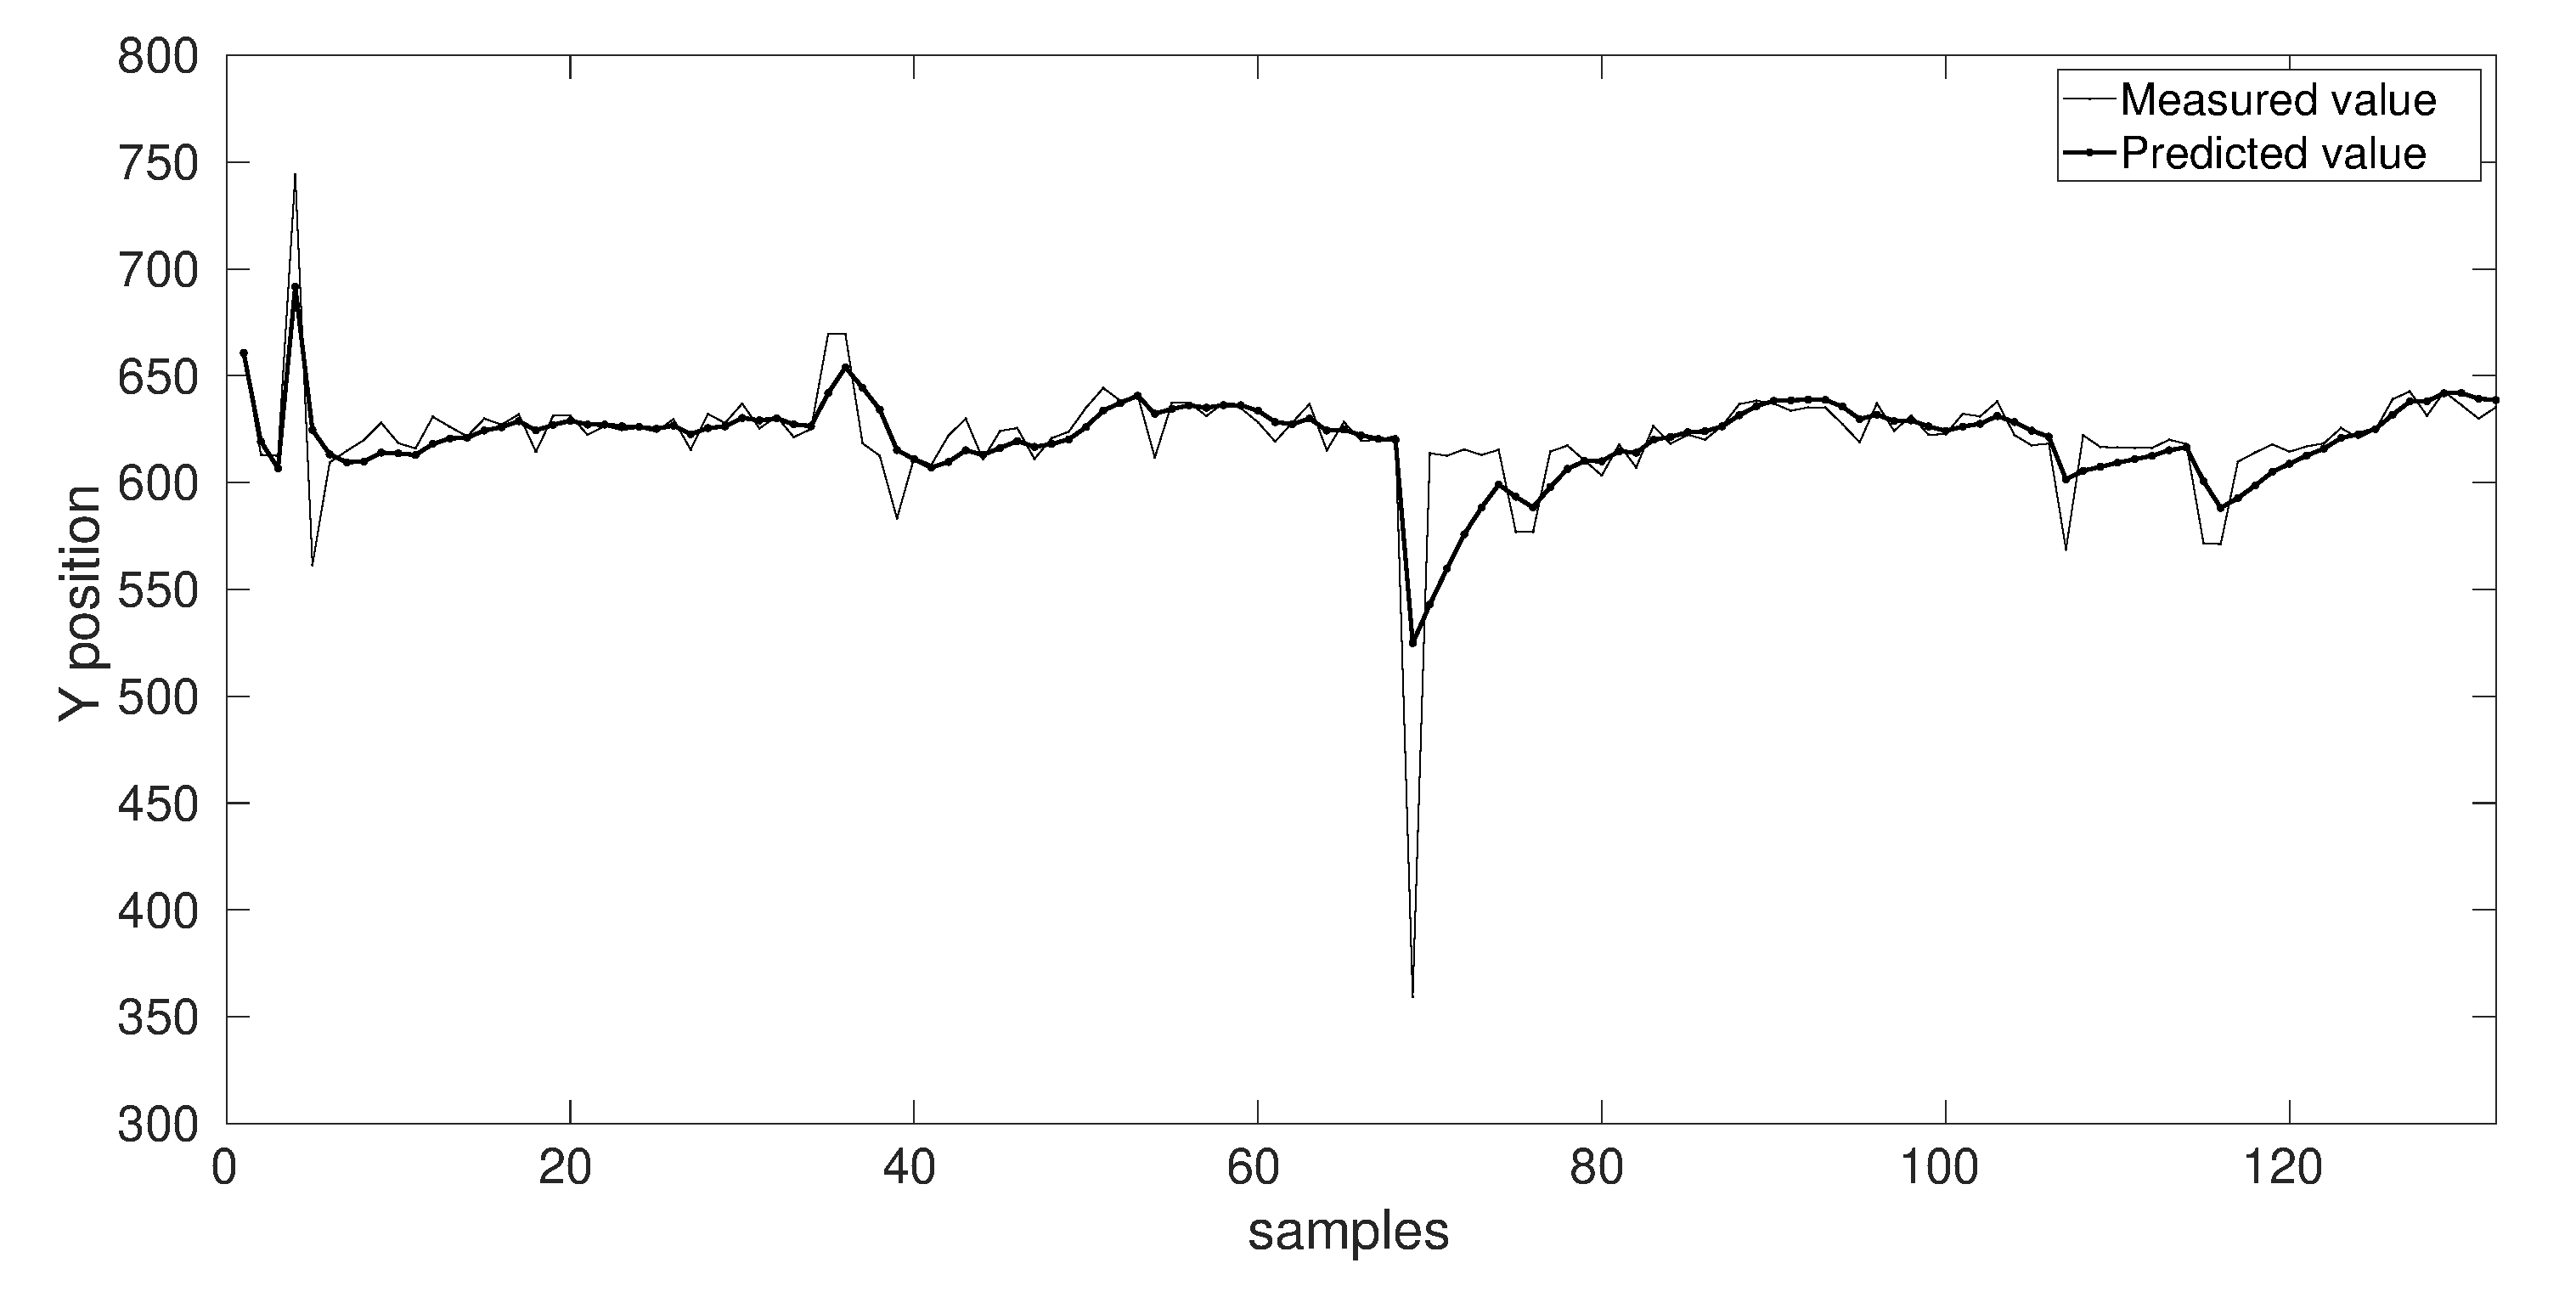
\includegraphics[width = \textwidth]{./Figures/part2Ratio1Y.eps}
	\caption{Kalman 2D Y-position plot for Ratio 1}
	\label{fig:kalman 2D YRat1}
\end{minipage}%%
\begin{minipage}{0.5\textwidth}
\centering
	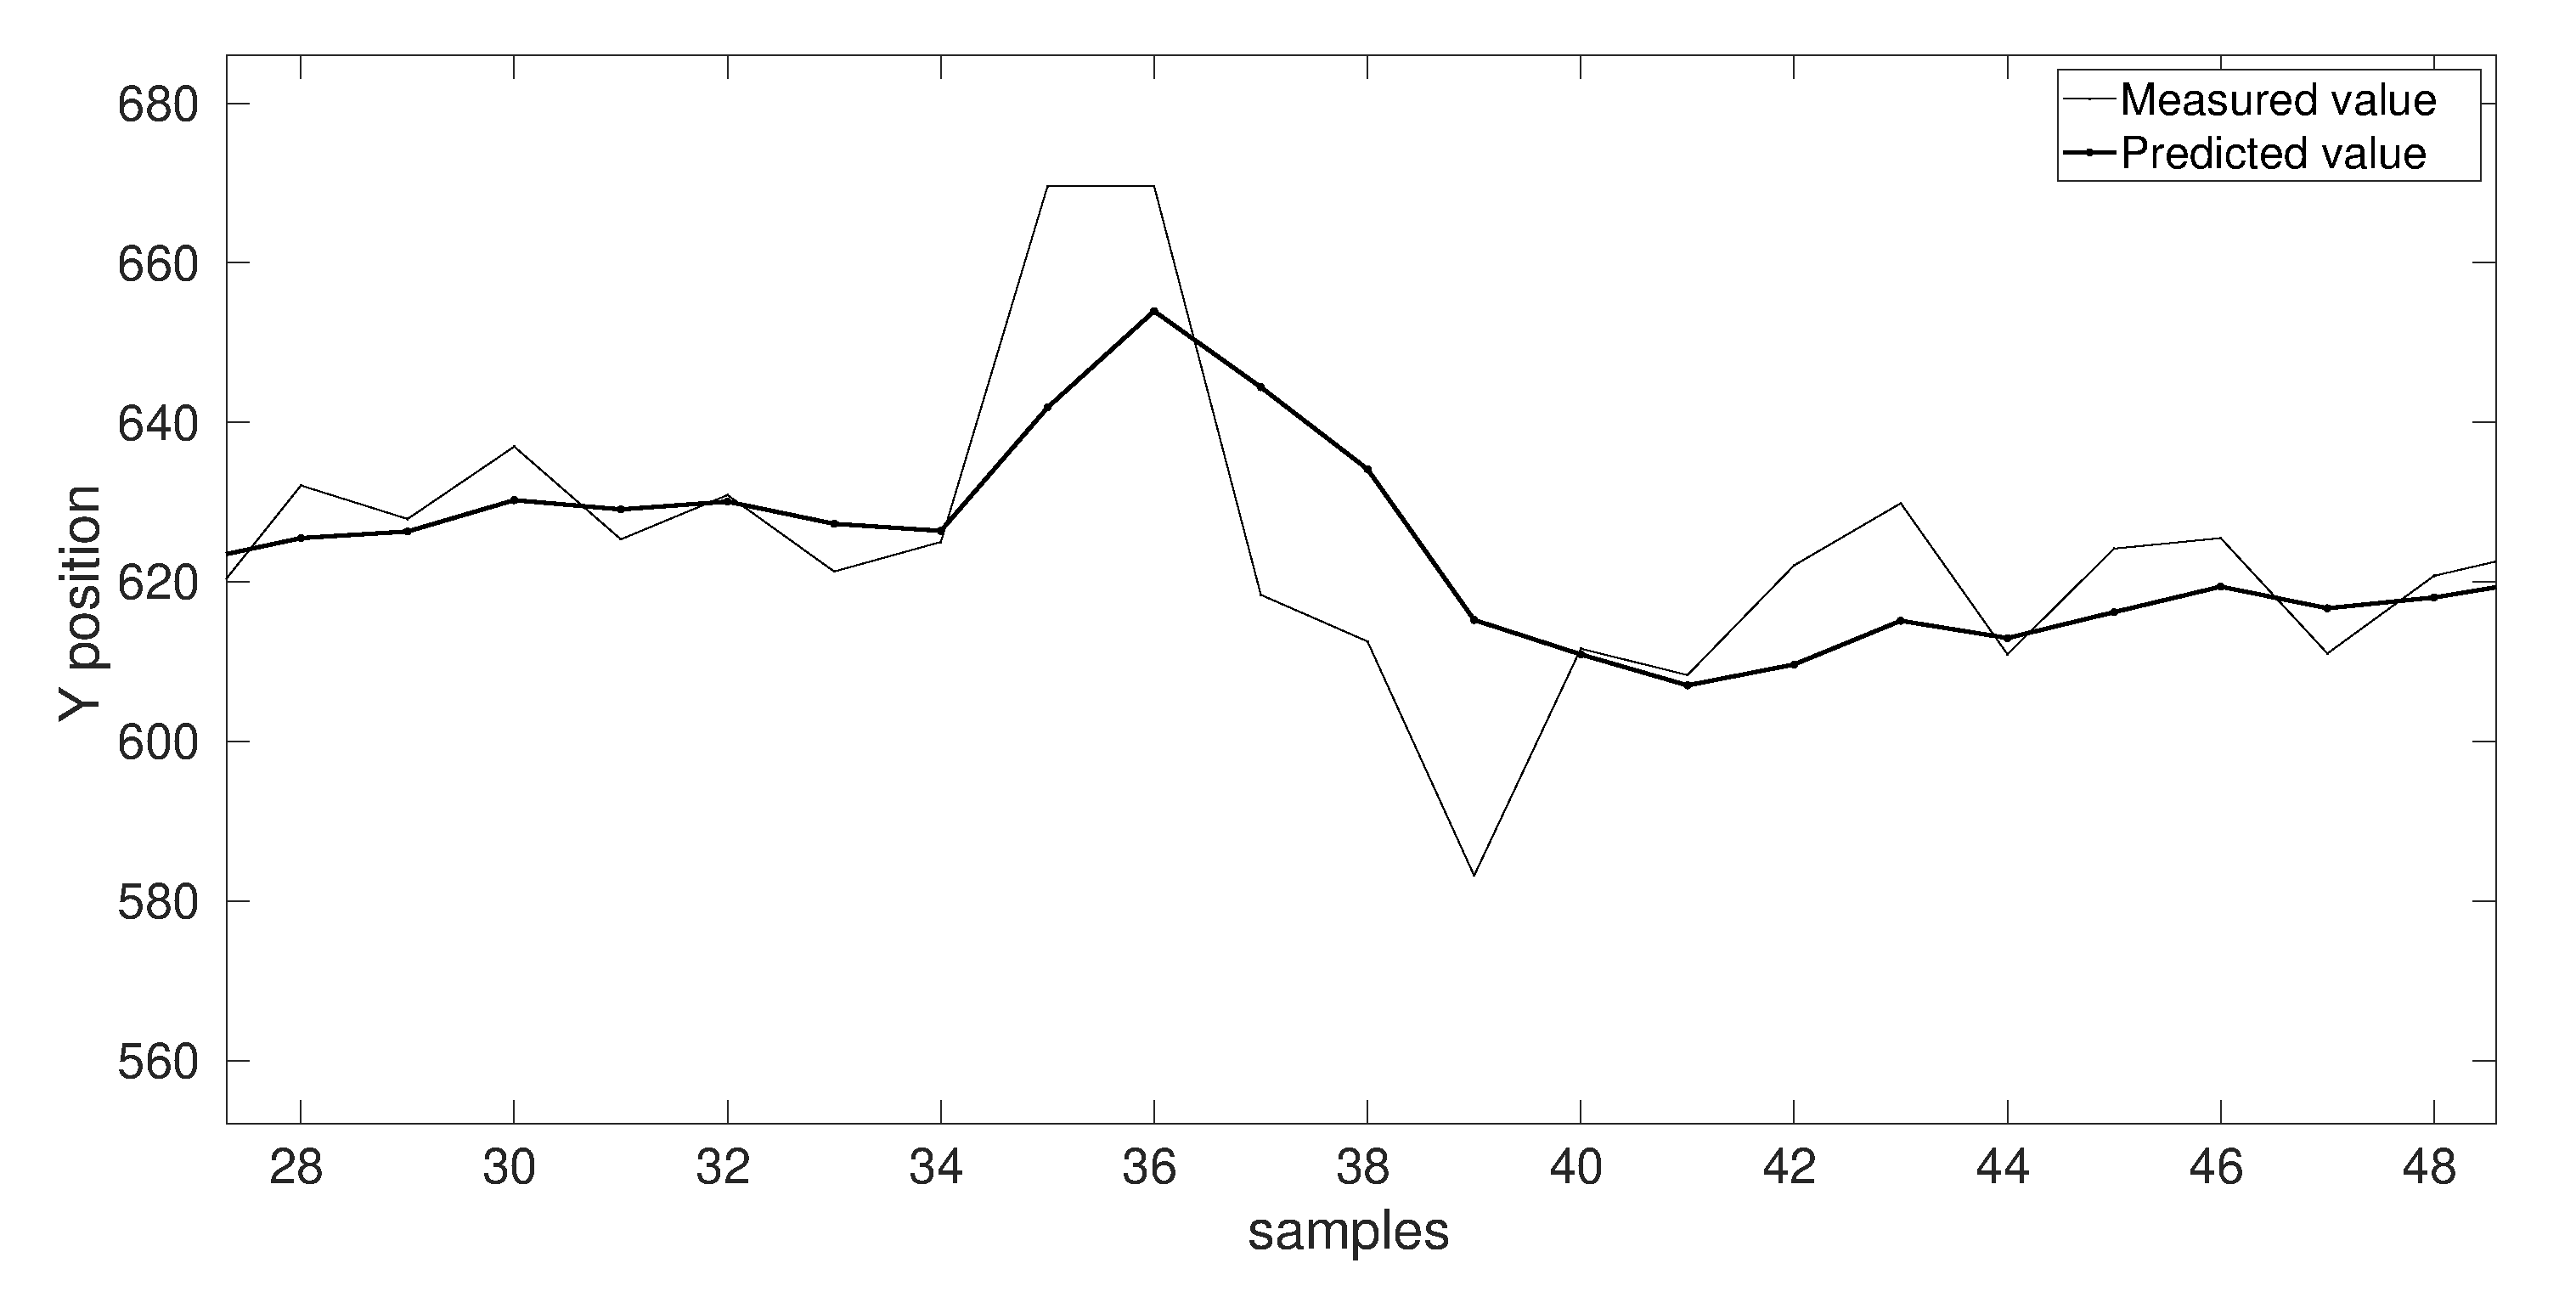
\includegraphics[width = \textwidth]{./Figures/part2Ratio1Yzoomed.eps}
	\caption{ Zoomed Y-position plot for Ratio 1}
	\label{fig: kalman 2D YRat1 zoom}
\end{minipage}
\end{figure}

%RAtio 2 0.01:0.001
\begin{figure}[hb!]
\centering
\begin{minipage}{0.5\textwidth}
\centering
	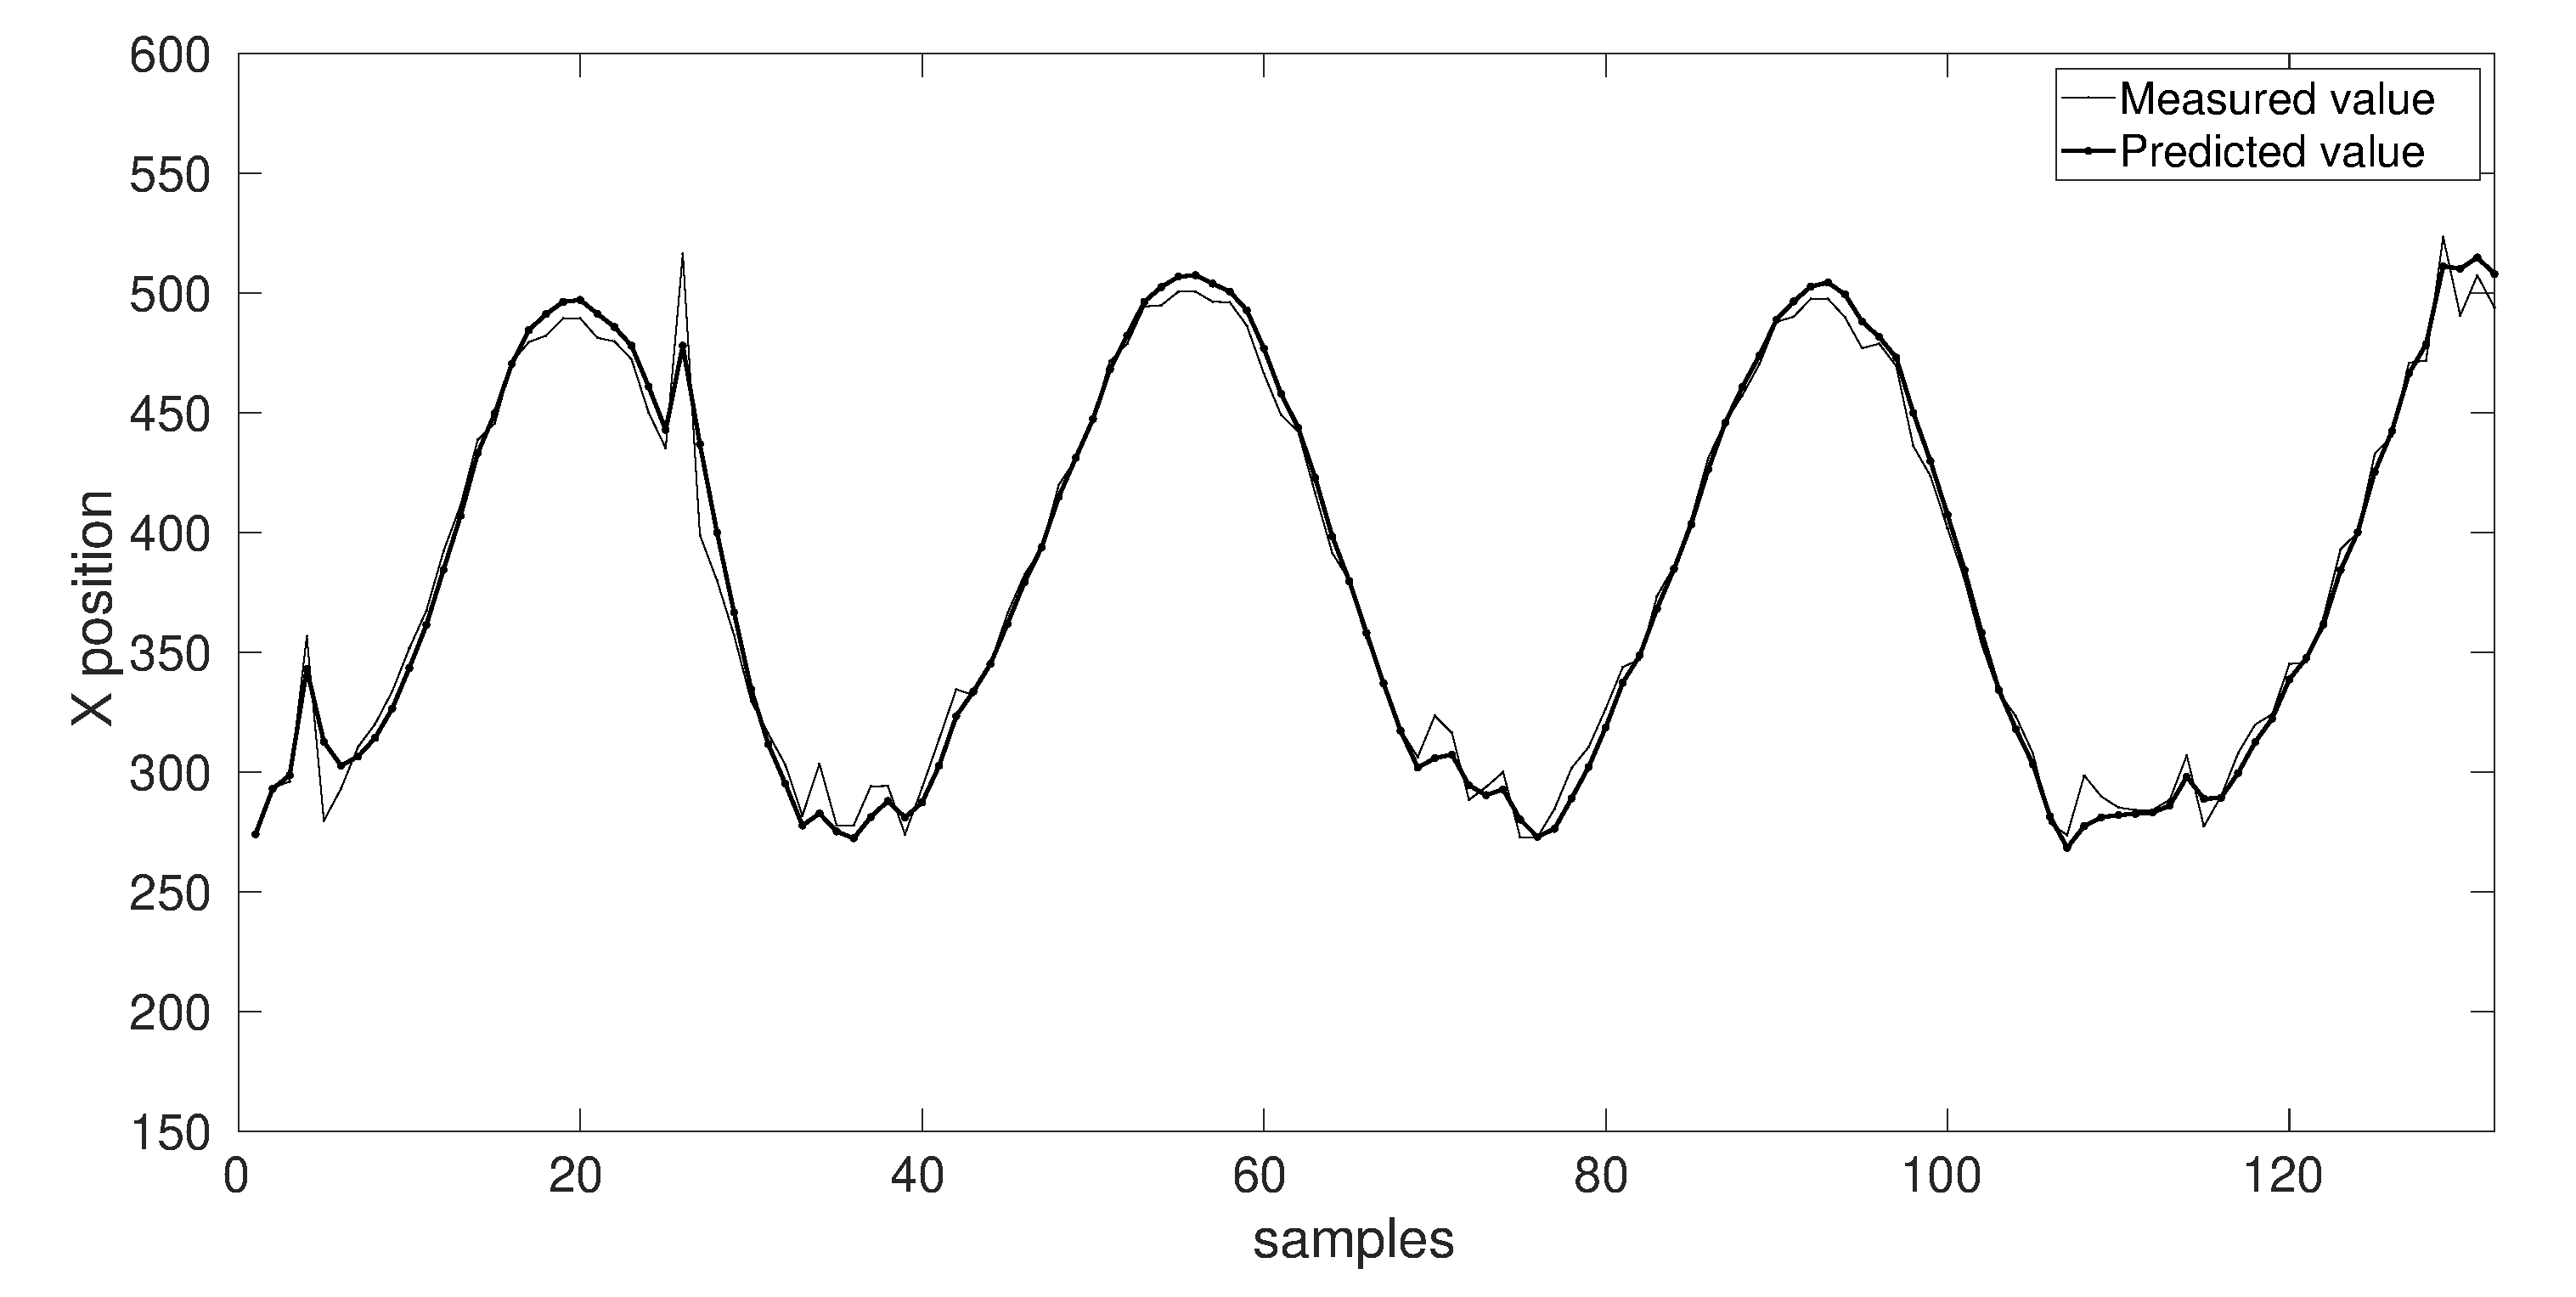
\includegraphics[width = \textwidth]{./Figures/part2Ratio2X.eps}
	\caption{Kalman 2D X-position Ratio 2 plot }
	\label{fig:kalman 2D XRat2}
\end{minipage}%%
\begin{minipage}{0.5\textwidth}
\centering
	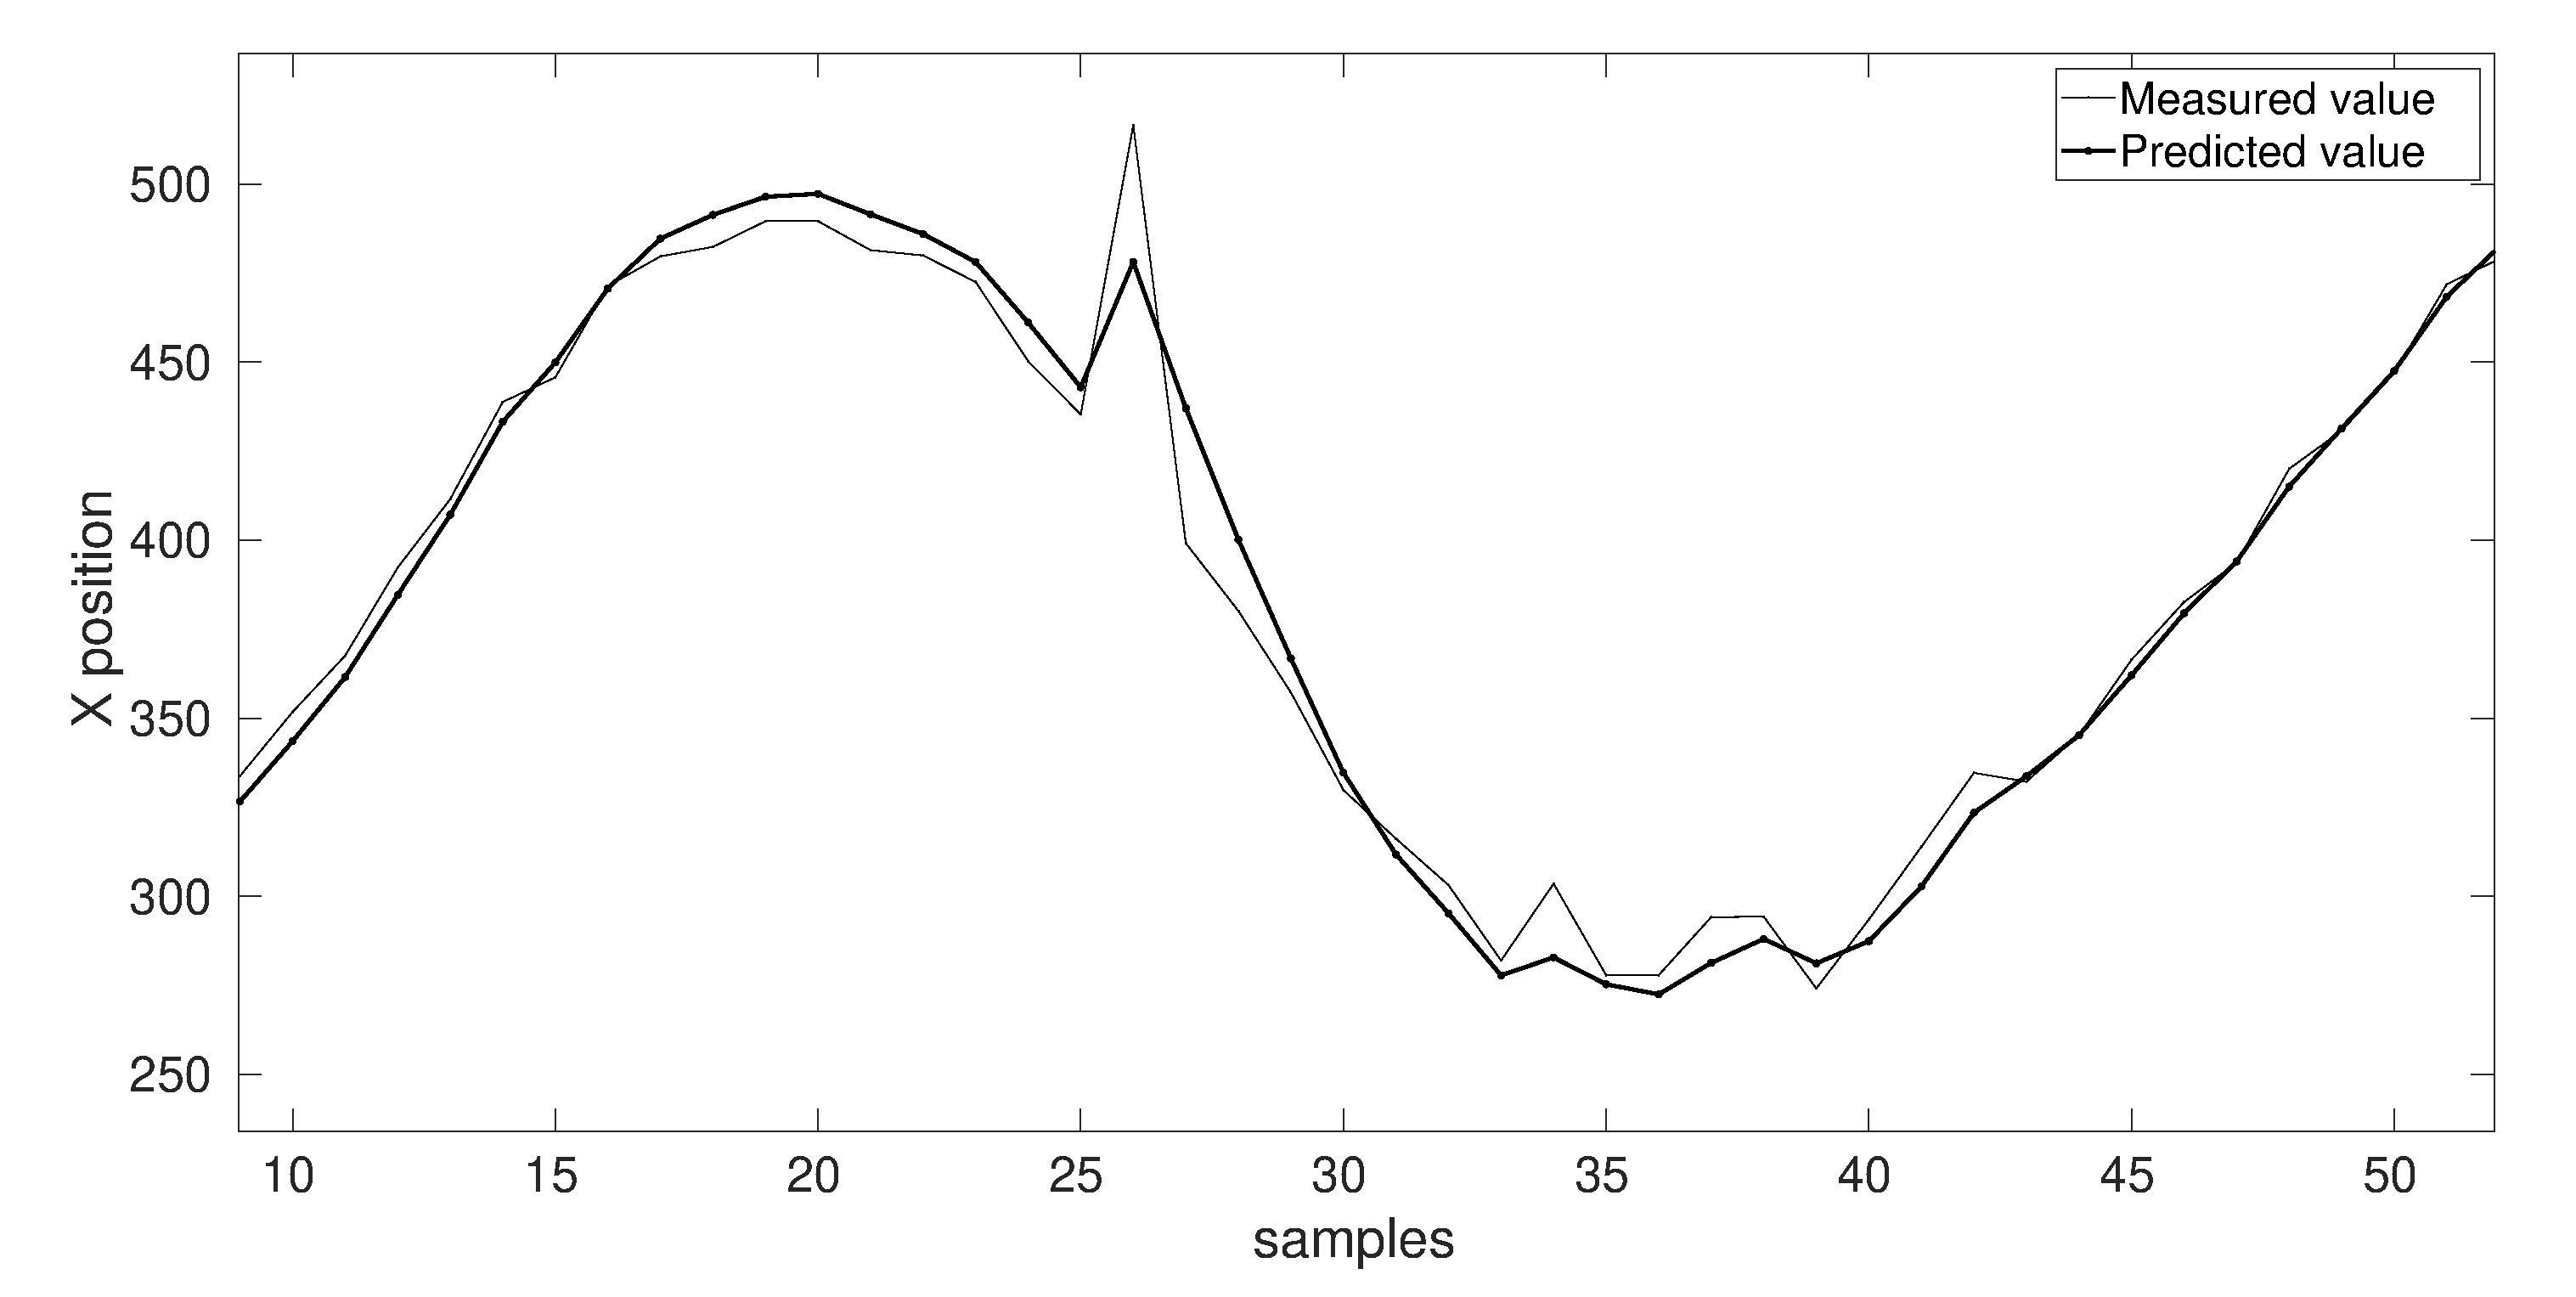
\includegraphics[width = \textwidth]{./Figures/part2Ratio2Xzoomed.eps}
	\caption{ Zoomed X-position plot for Ratio 2}
	\label{fig: kalman 2D XRat2 zoom}
\end{minipage}
\begin{minipage}{0.5\textwidth}
\centering
	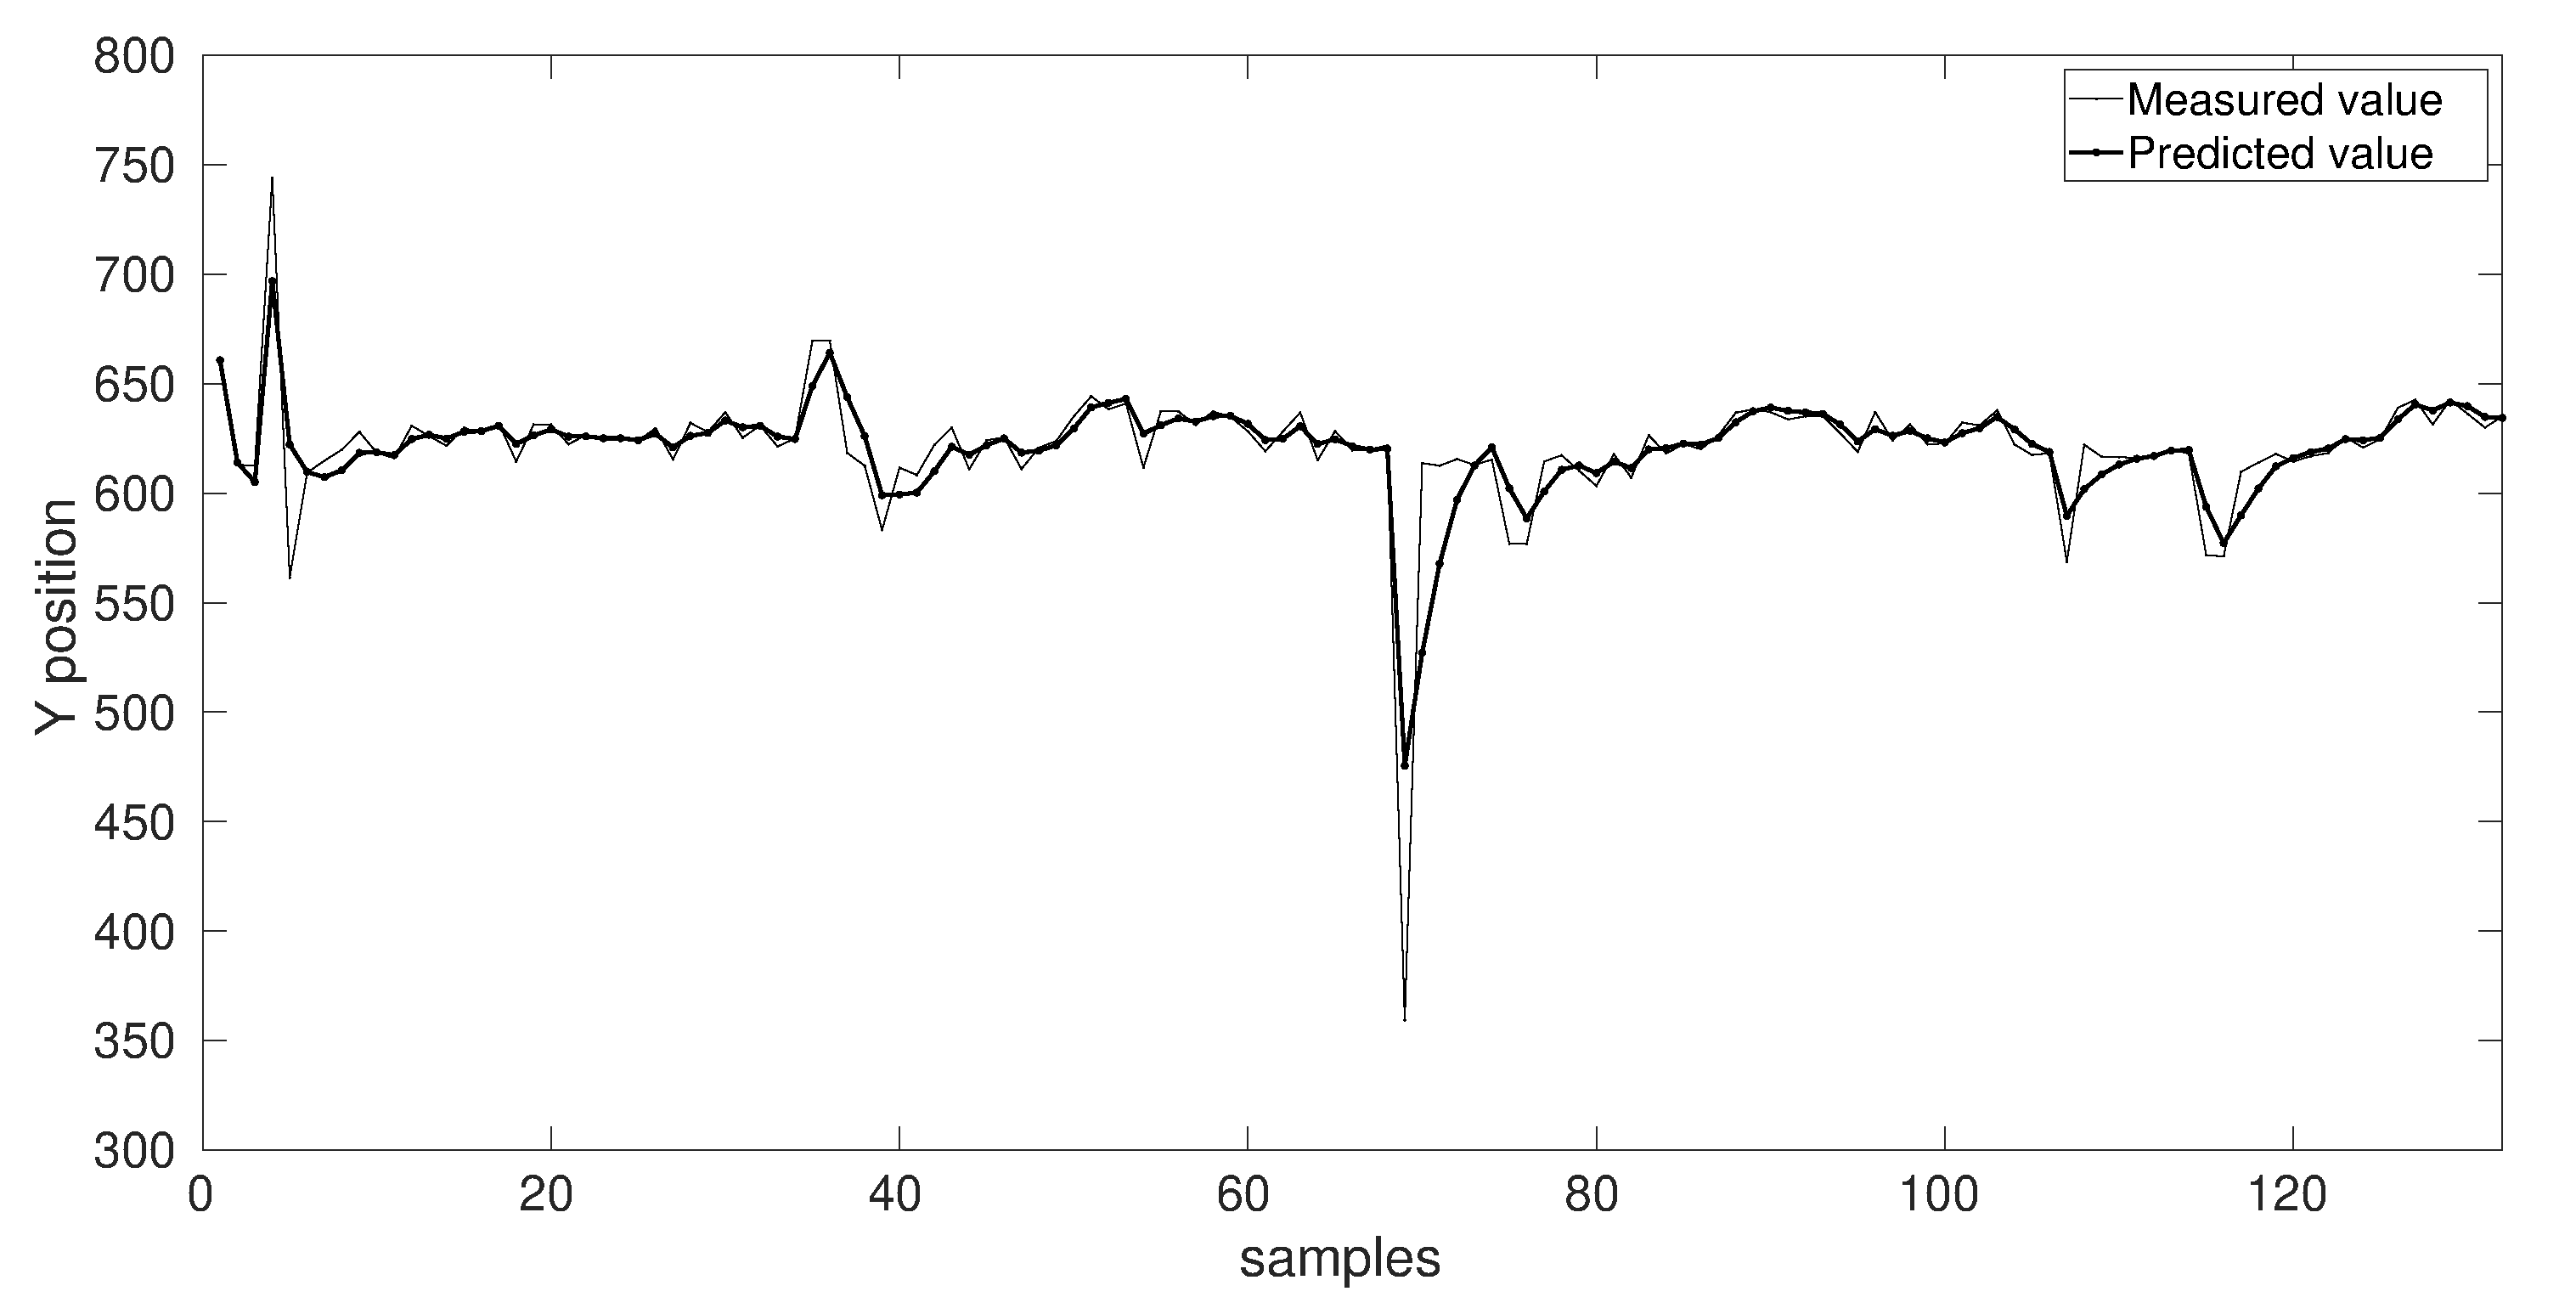
\includegraphics[width = \textwidth]{./Figures/part2Ratio2Y.eps}
	\caption{Kalman 2D Y-position Ratio 2 plot }
	\label{fig:kalman 2D YRat2}
\end{minipage}%%
\begin{minipage}{0.5\textwidth}
\centering
	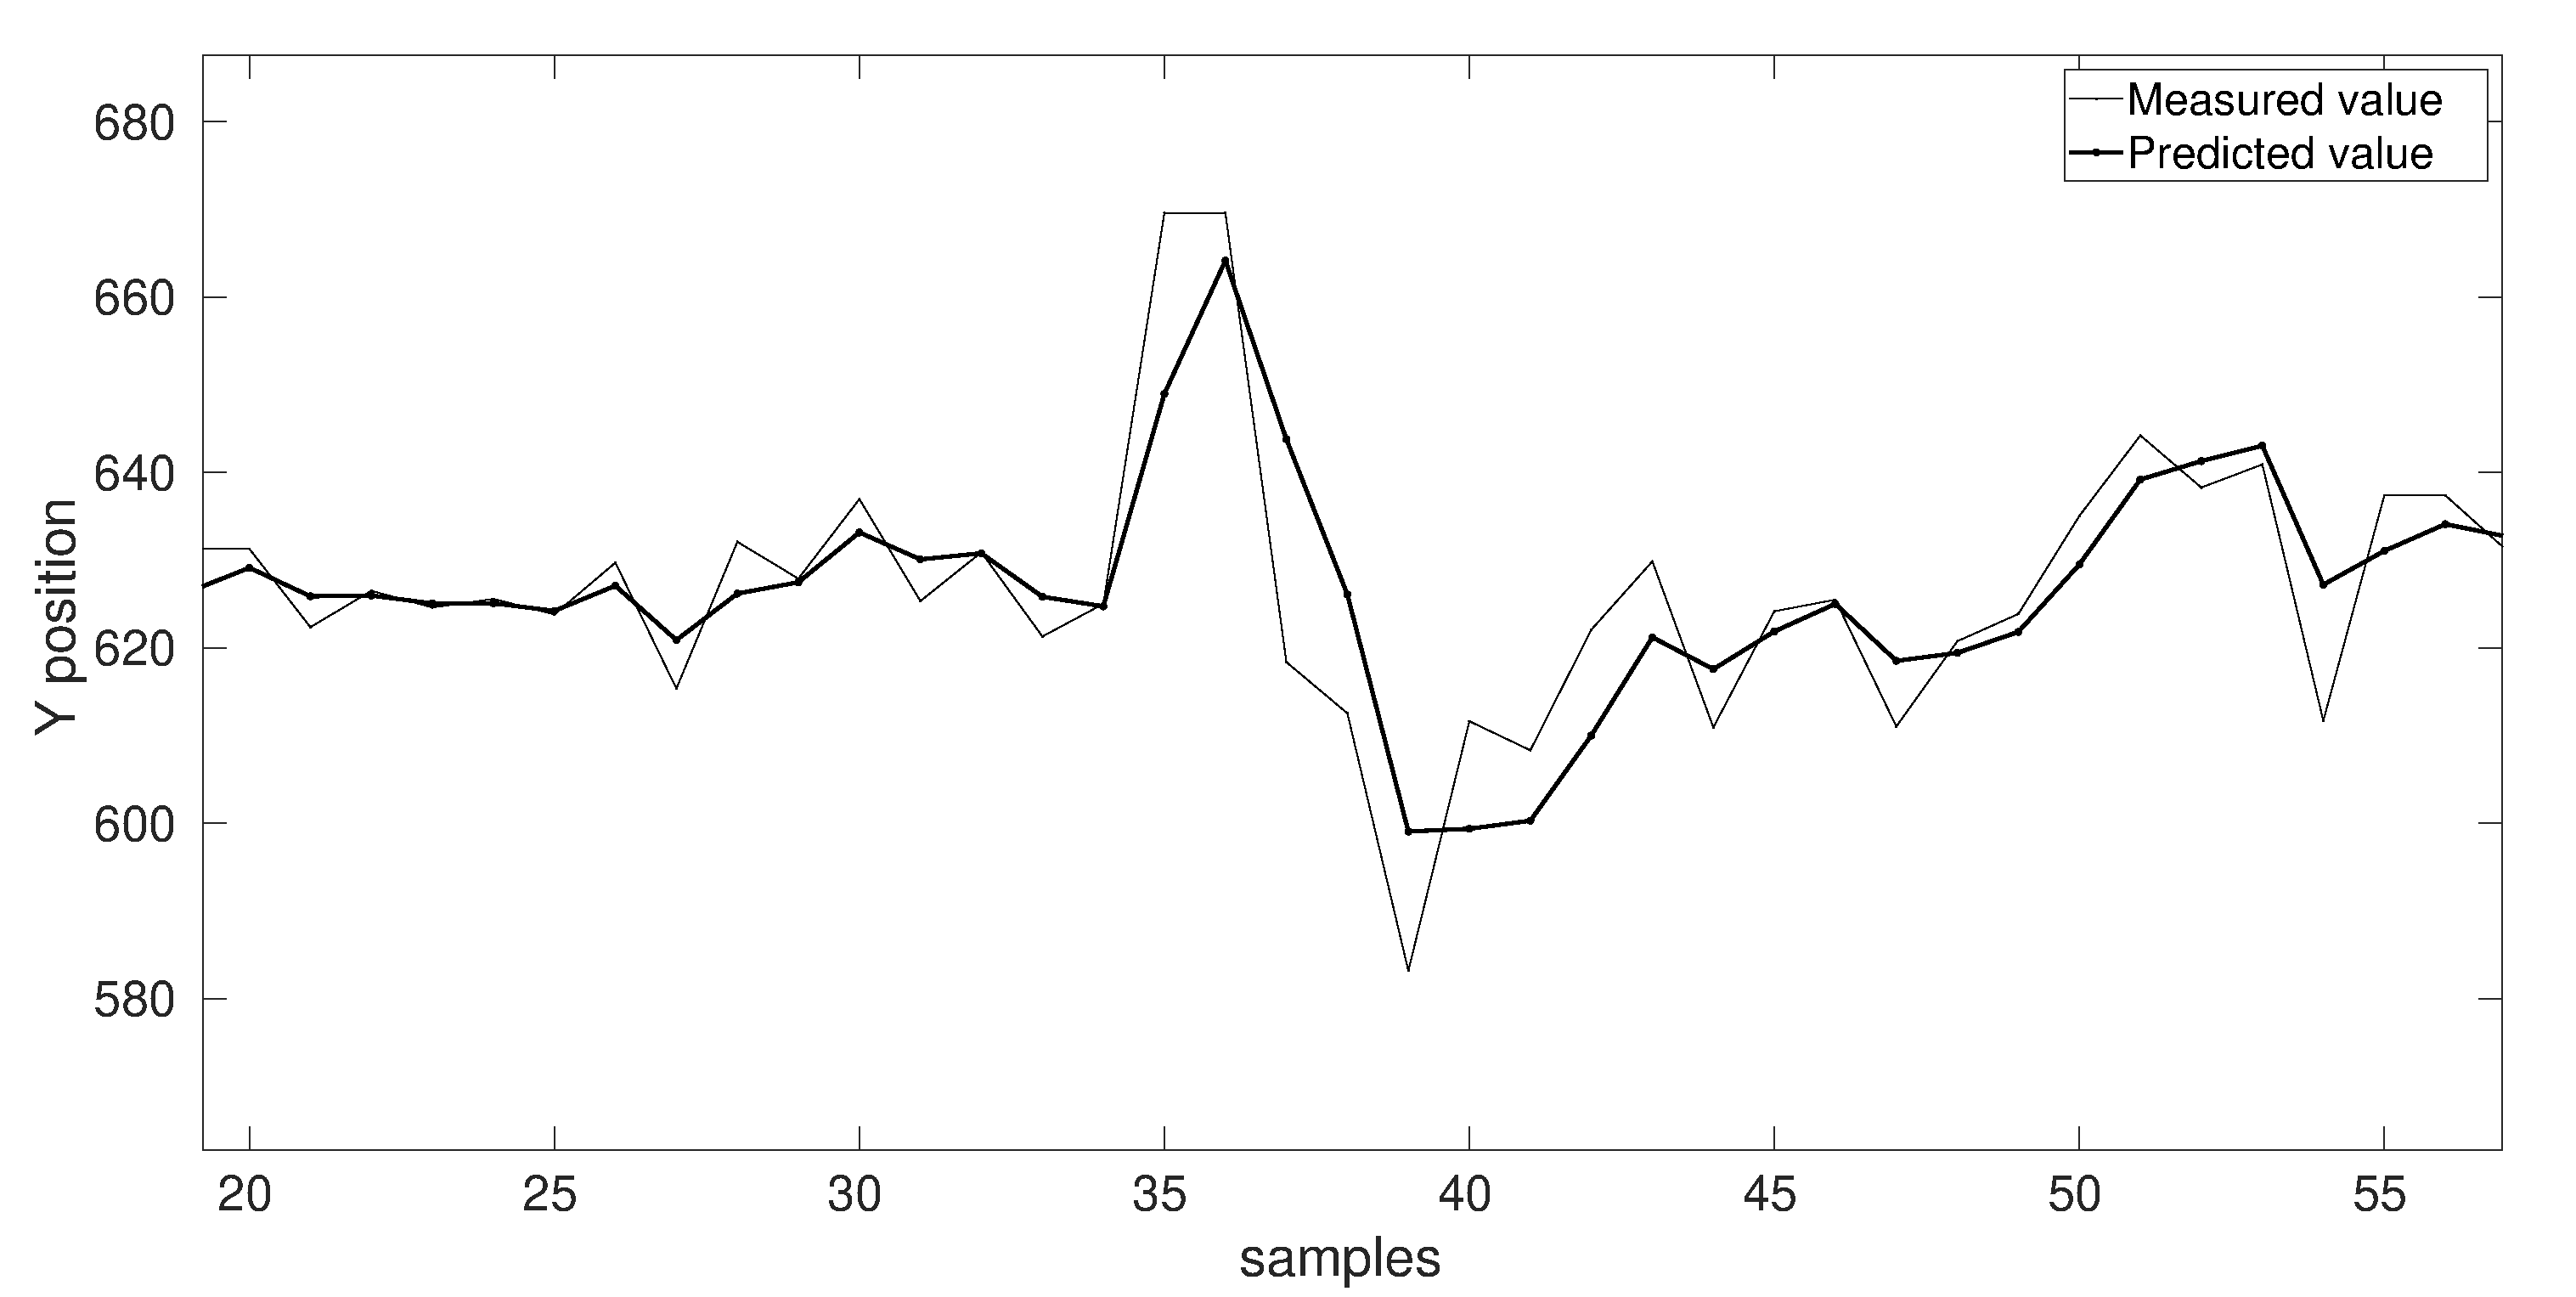
\includegraphics[width = \textwidth]{./Figures/part2Ratio2Yzoomed.eps}
	\caption{ Zoomed Y-position plot for Ratio 2}
	\label{fig: kalman 2D YRat2 zoom}
\end{minipage}
\end{figure}

\newpage
%RAtio 3 0.001:0.h01
\begin{figure}[ht!]
\centering
\begin{minipage}{0.5\textwidth}
\centering
	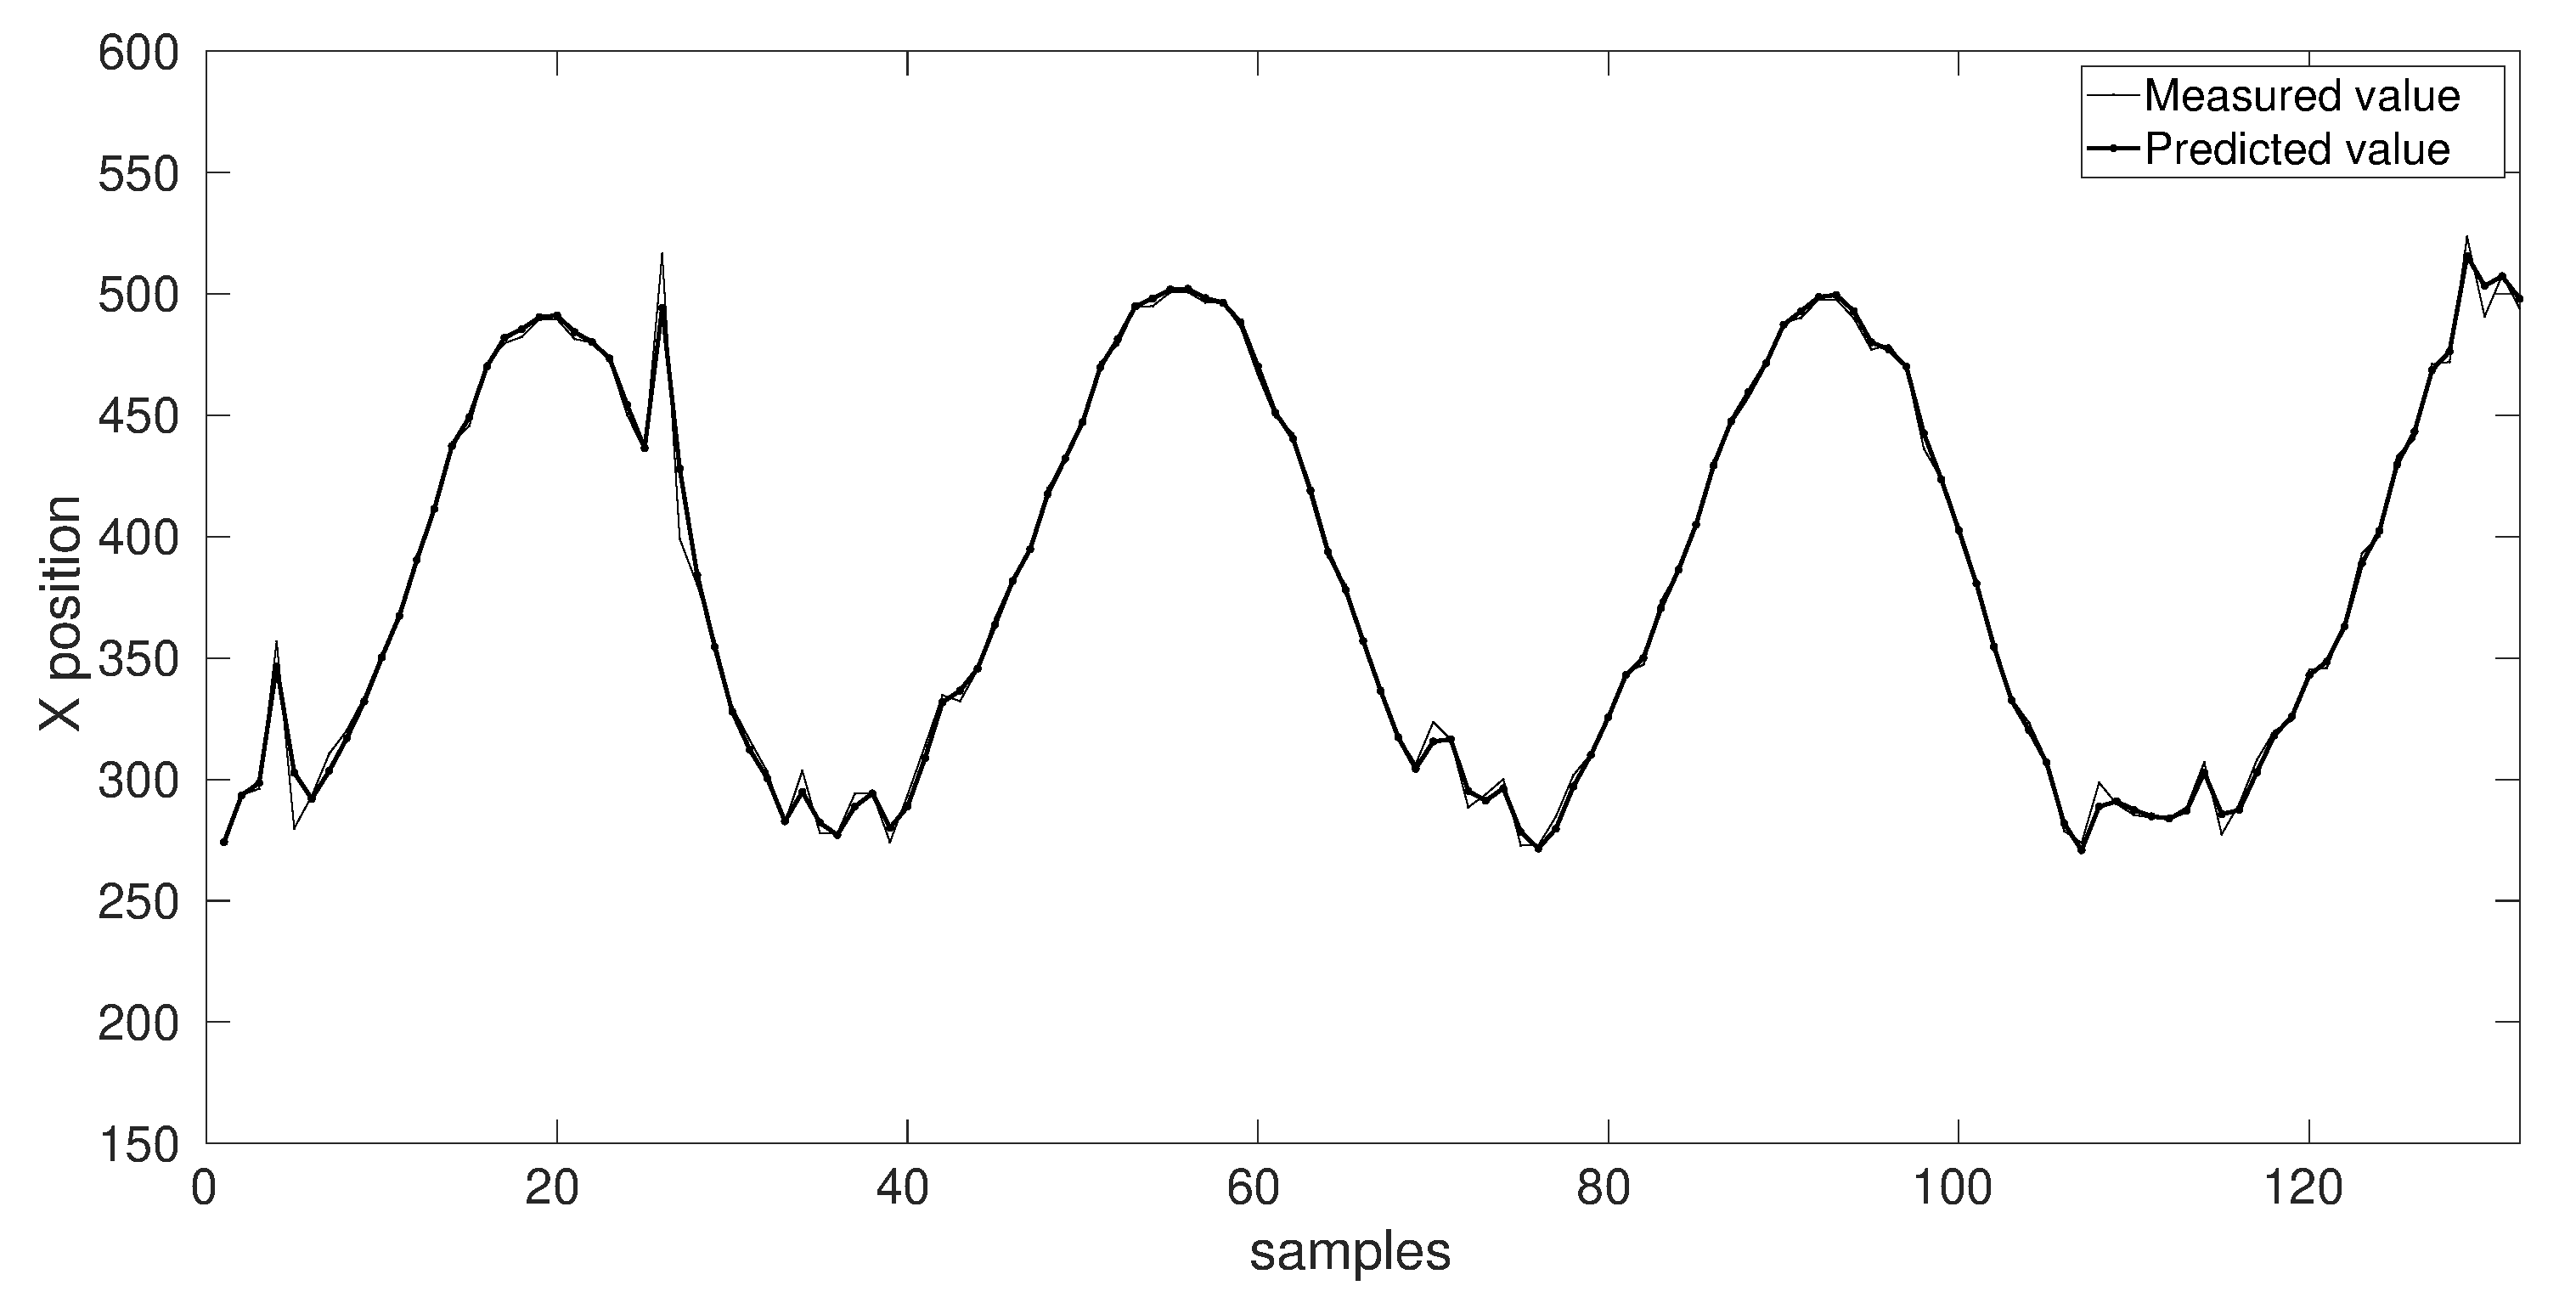
\includegraphics[width = \textwidth]{./Figures/part2Ratio3X.eps}
	\caption{Kalman 2D X-position Ratio 3 plot }
	\label{fig:kalman 2D XRat3}
\end{minipage}%%
\begin{minipage}{0.5\textwidth}
\centering
	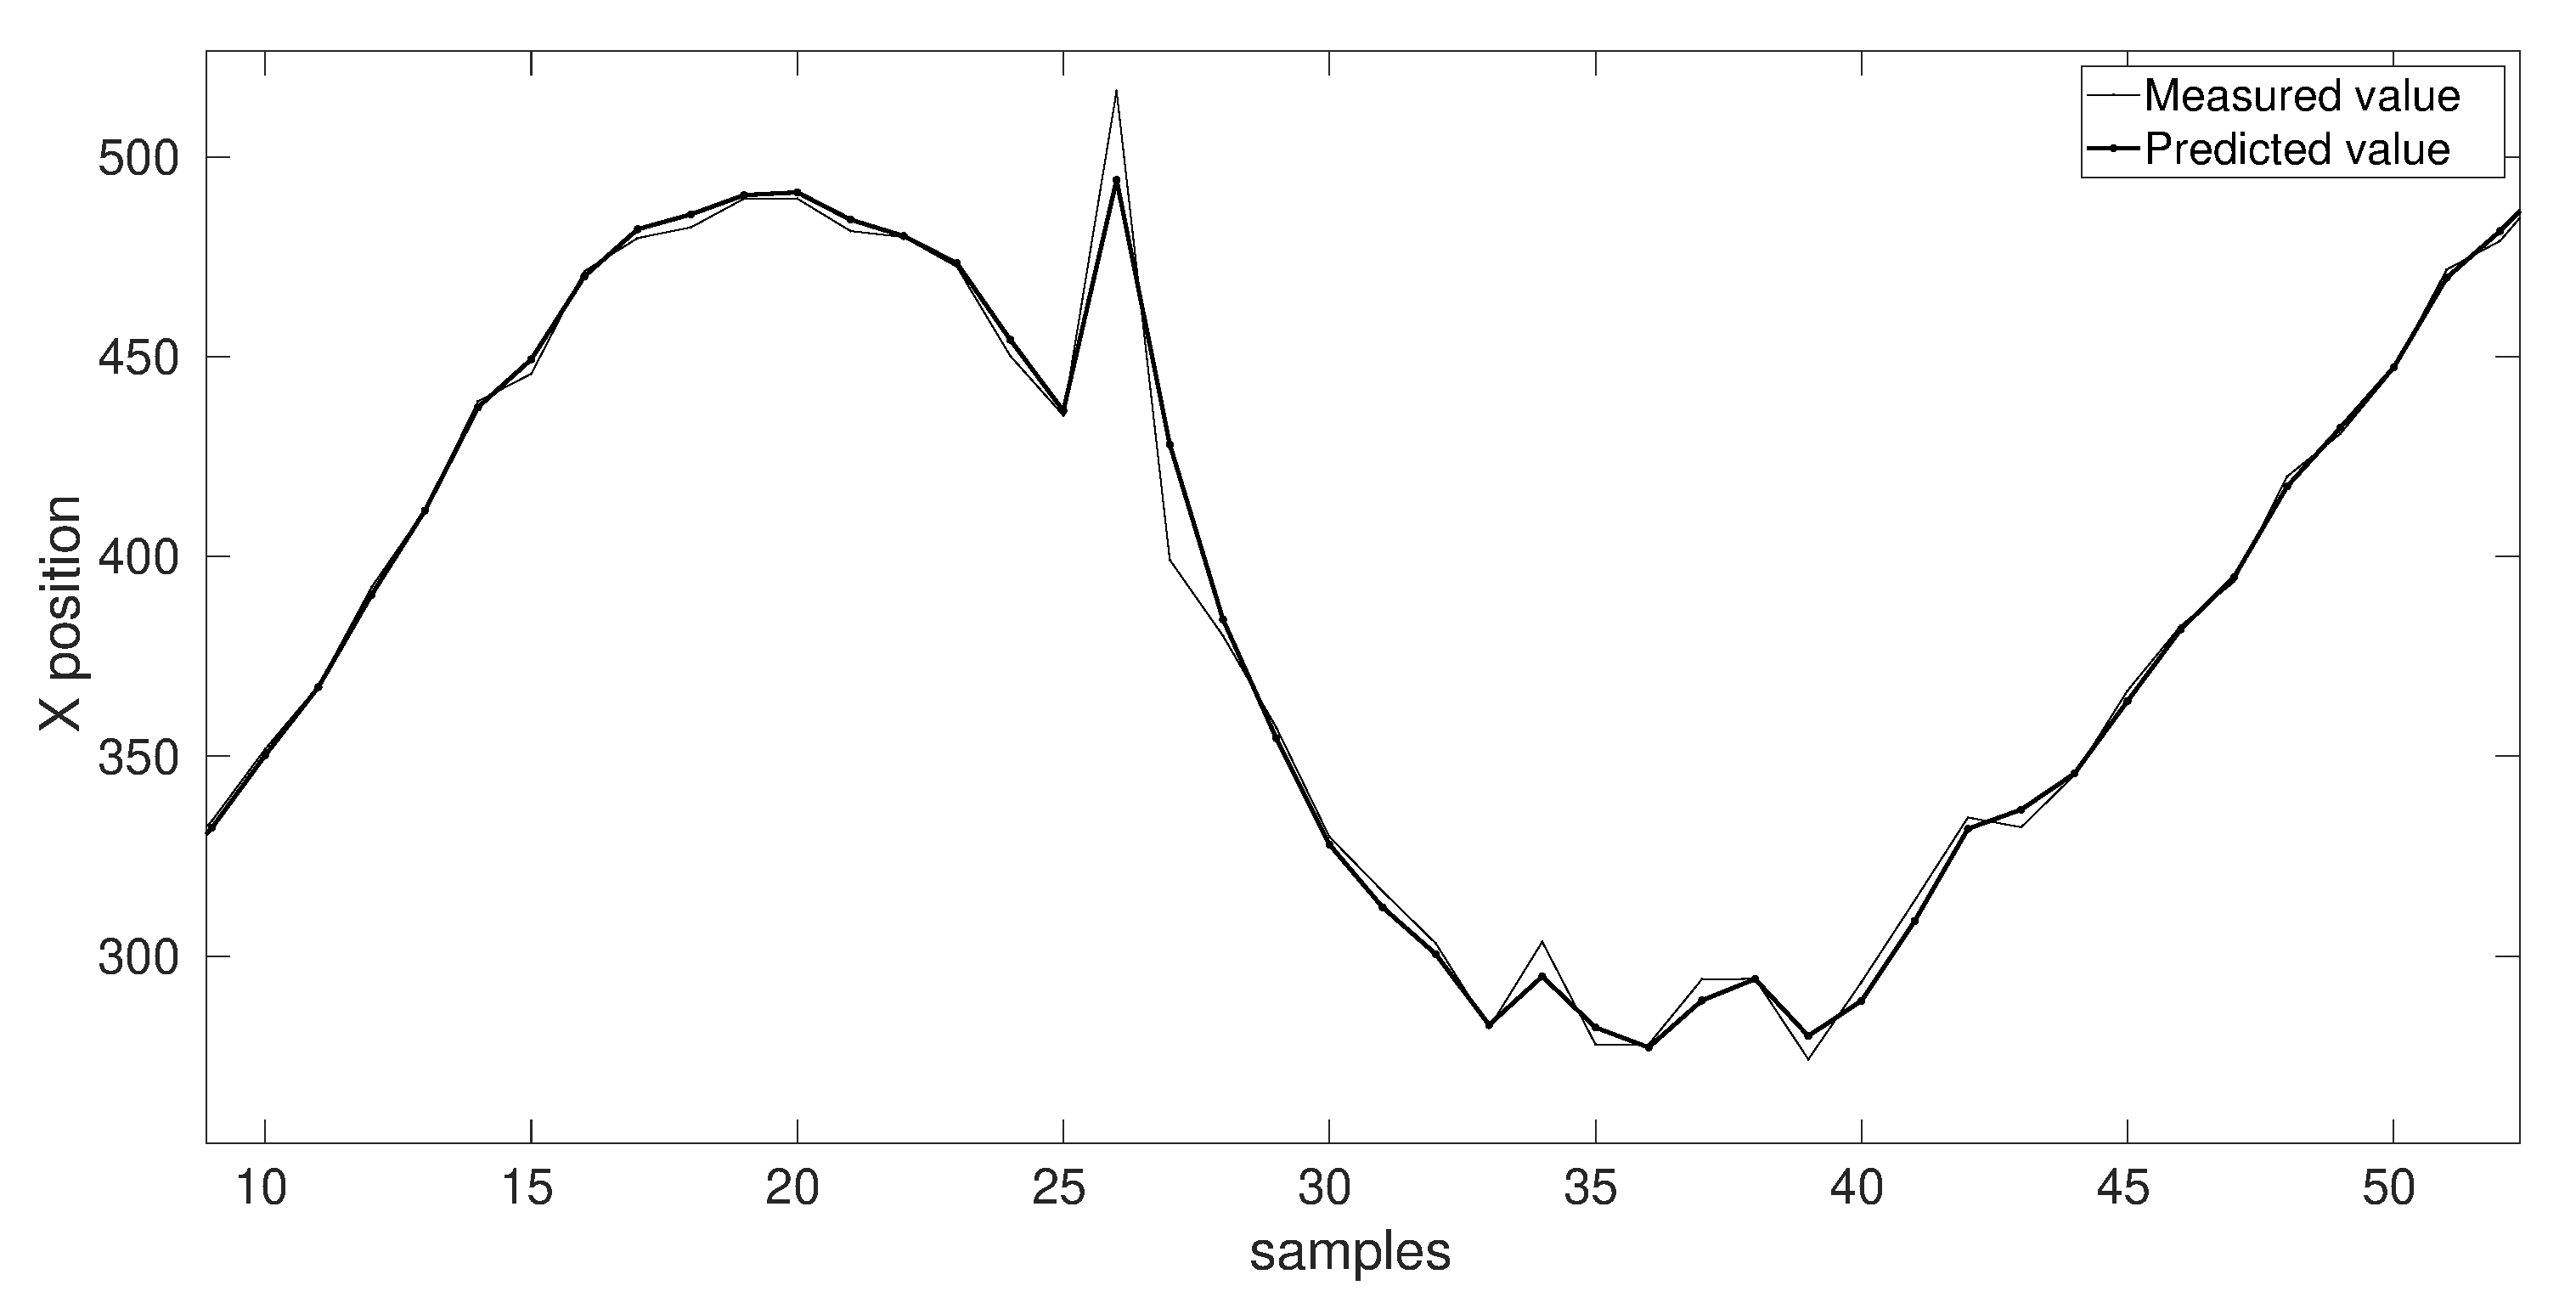
\includegraphics[width = \textwidth]{./Figures/part2Ratio3Xzoomed.eps}
	\caption{ Zoomed X-position plot for Ratio 3}
	\label{fig: kalman 2D XRat3 zoom}
\end{minipage}
\begin{minipage}{0.5\textwidth}
\centering
	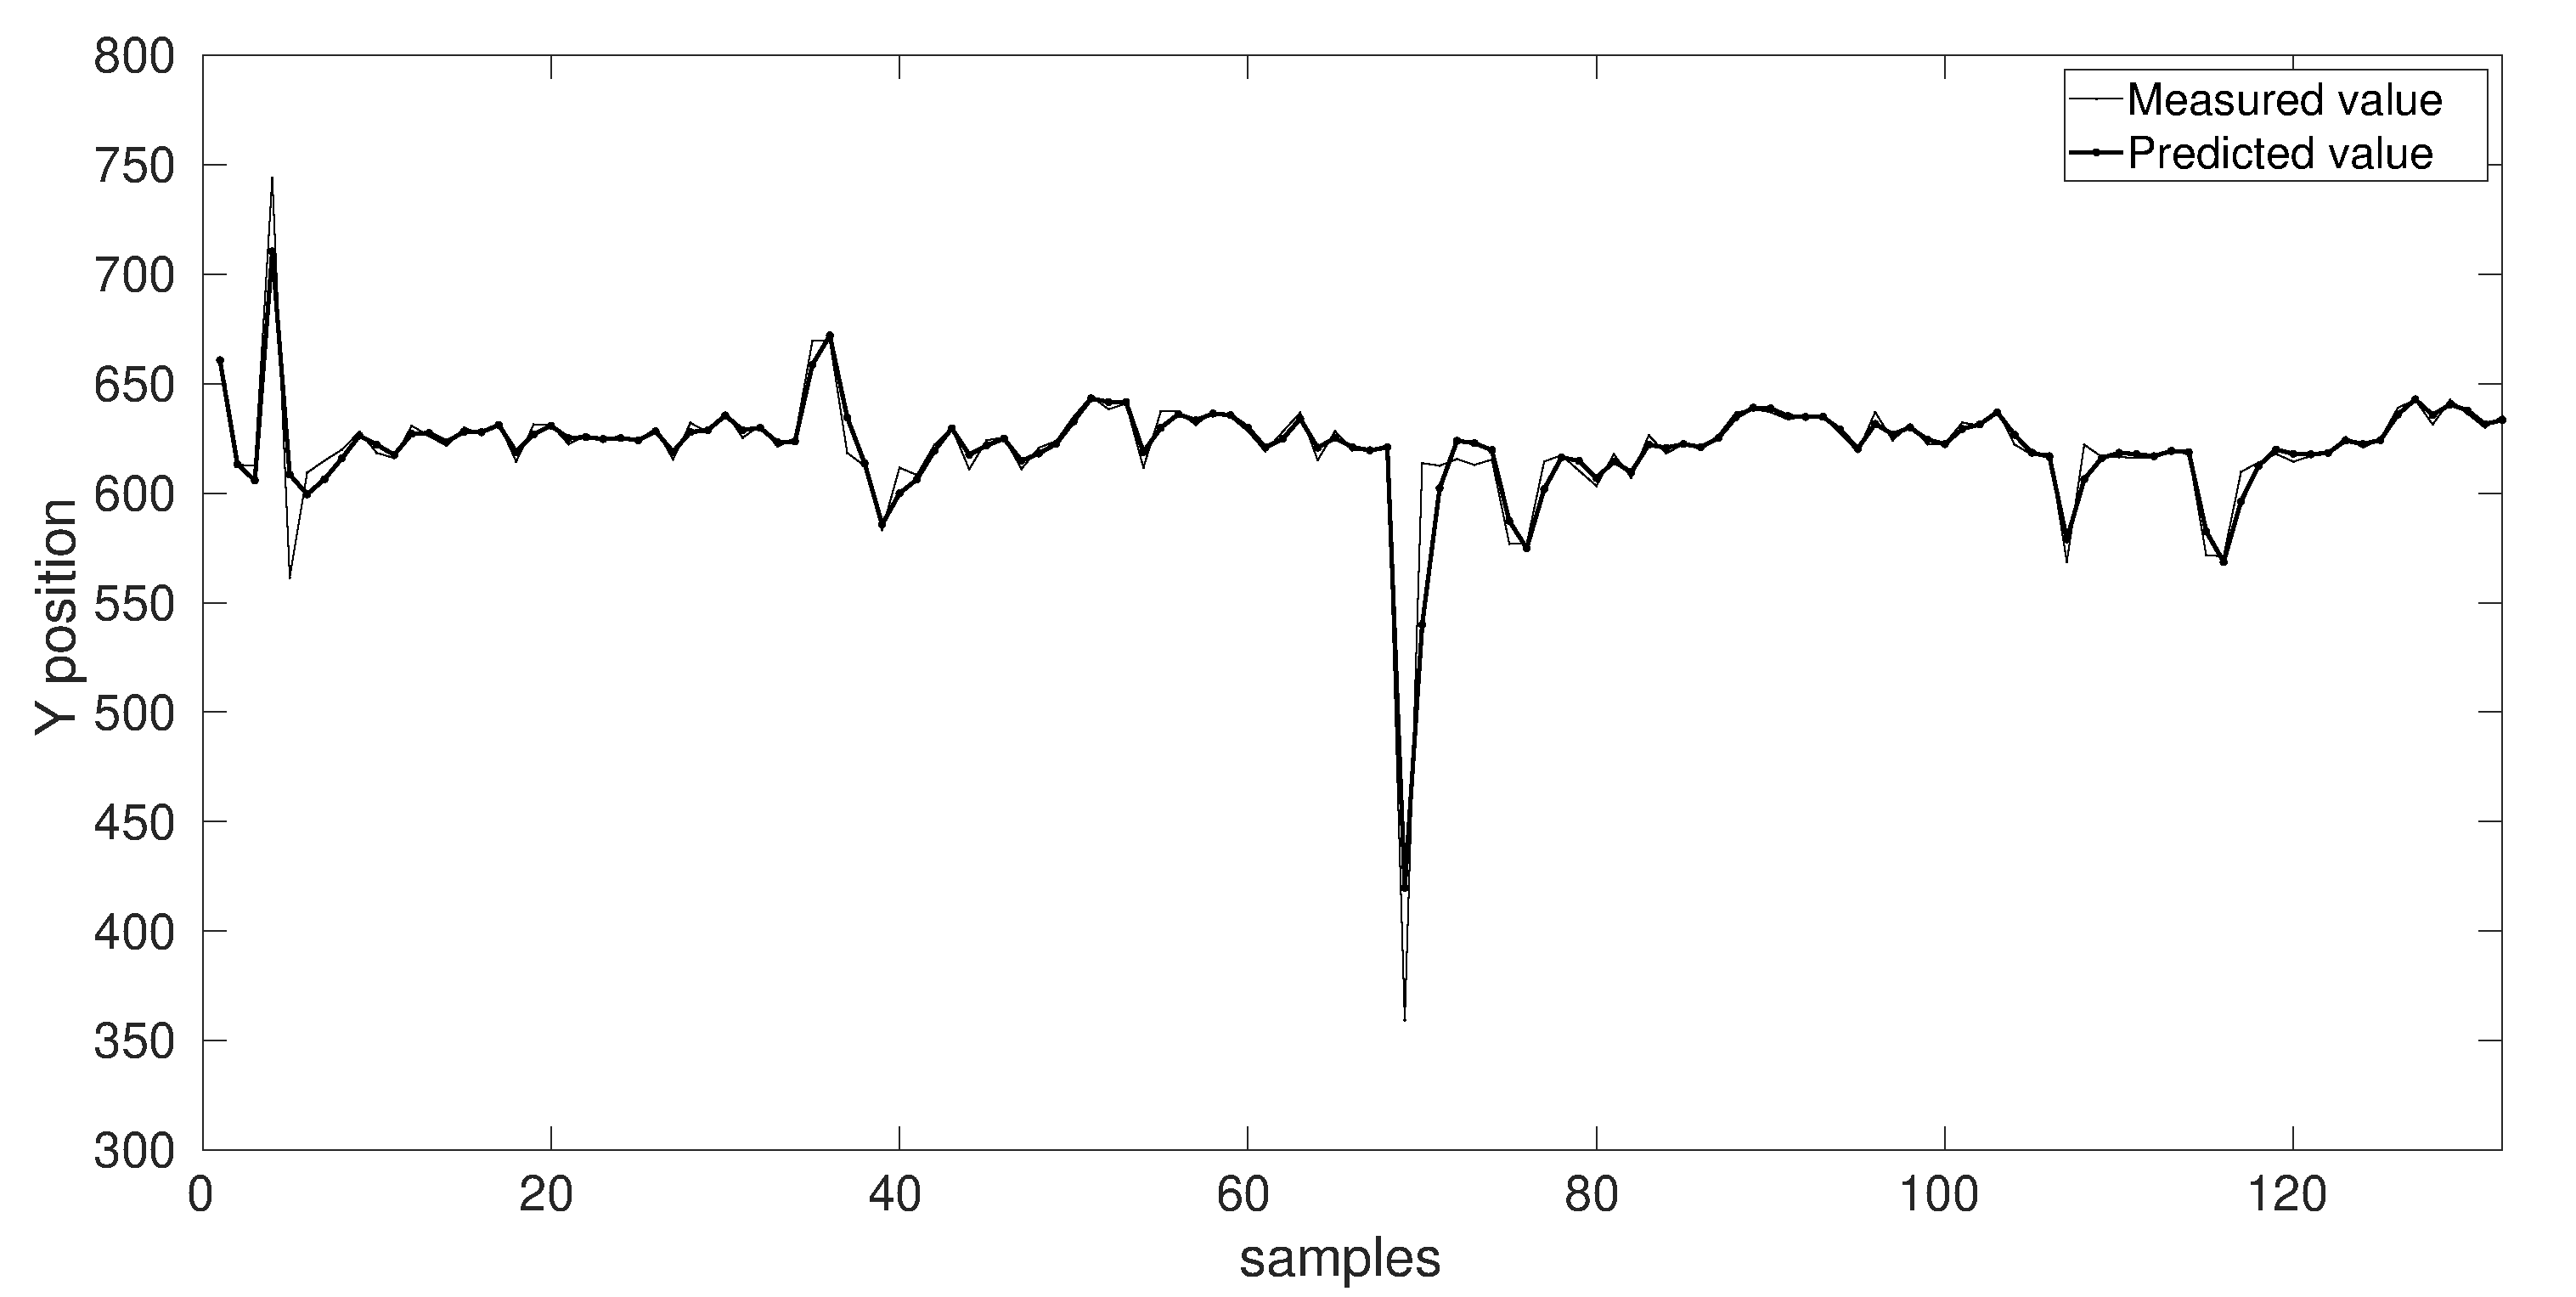
\includegraphics[width = \textwidth]{./Figures/part2Ratio3Y.eps}
	\caption{Kalman 2D Y-position Ratio 3 plot }
	\label{fig:kalman 2D YRat3}
\end{minipage}%%
\begin{minipage}{0.5\textwidth}
\centering
	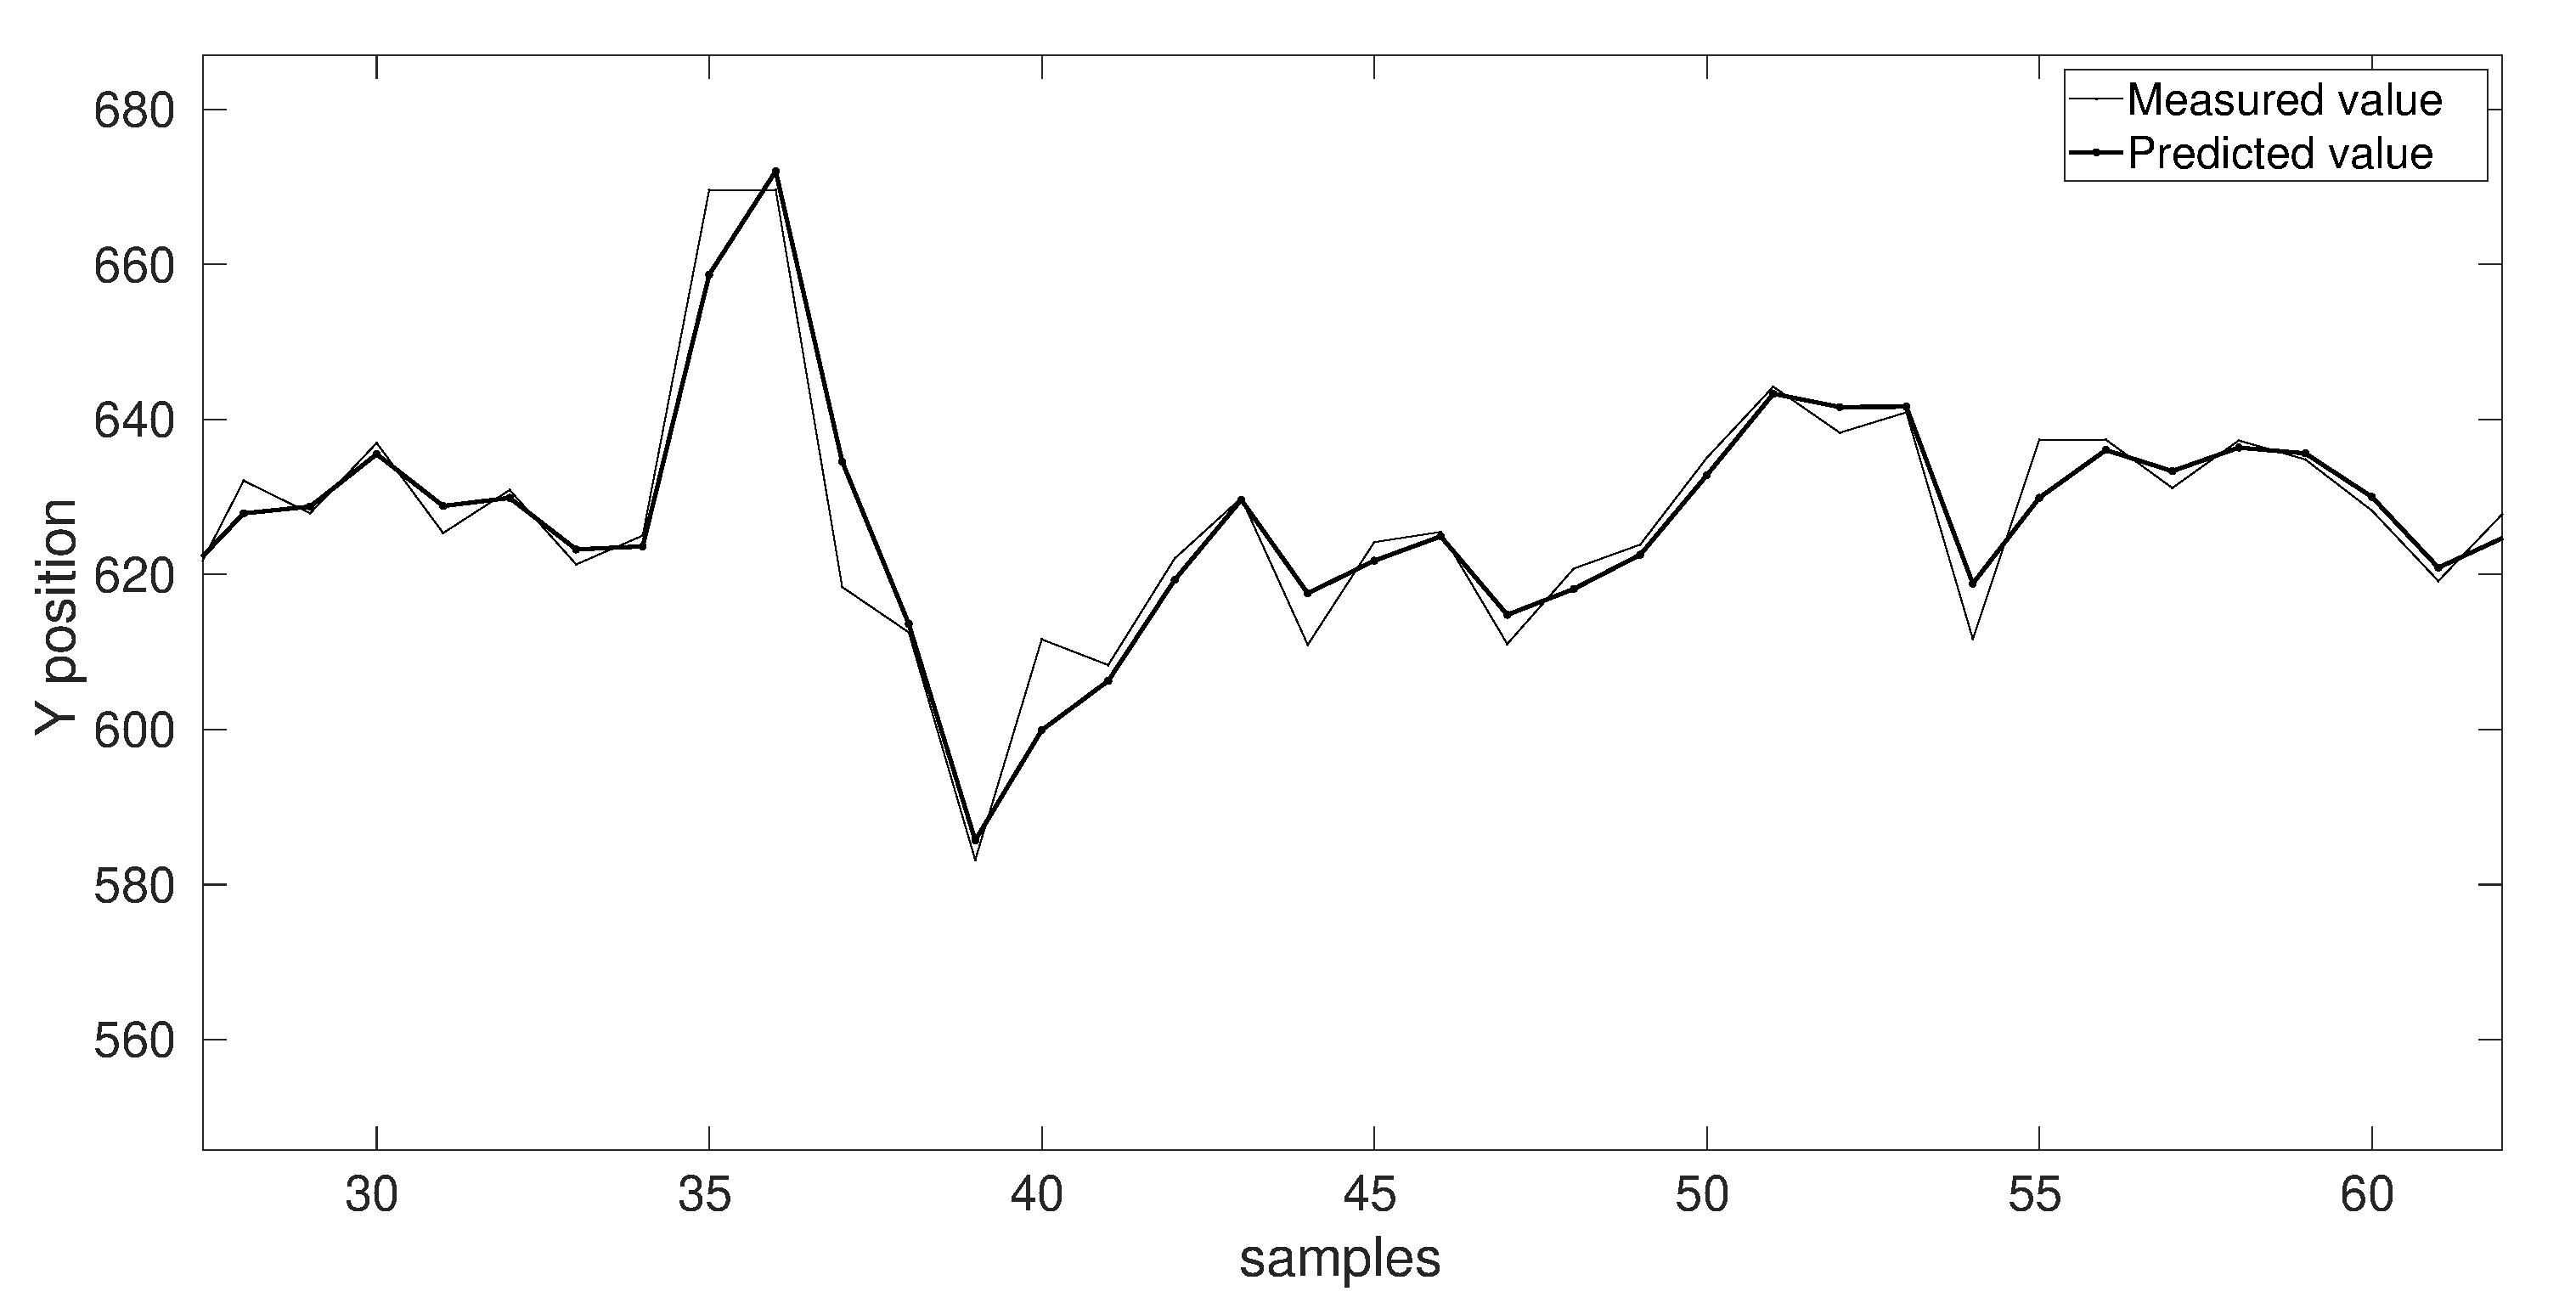
\includegraphics[width = \textwidth]{./Figures/part2Ratio3Yzoomed.eps}
	\caption{ Zoomed Y-position plot for Ratio 3}
	\label{fig: kalman 2D YRat3 zoom}
\end{minipage}
\end{figure}
\quad \\
\noindent
Figure \ref{fig:kalman 2D XRat1} and Figure \ref{fig:kalman 2D YRat1} represents the X-position and Y-position plot of the 2D dataset and the Kalman filter prediction. For this plot Ratio 1 i.e.\textbf{Measurement noise(R) = 0.1} and \textbf{dynamic noise(Q) = 0.001} is considered.\\
\\
\noindent
Figure \ref{fig:kalman 2D XRat2} and Figure \ref{fig:kalman 2D YRat2} represents the X-position and Y-position plot of the 2D dataset and the Kalman filter prediction. For this plot Ratio 2 i.e.\textbf{Measurement noise(R) = 0.01} and \textbf{dynamic noise(Q) = 0.001} is considered.\\
\\
\noindent
Figure \ref{fig:kalman 2D XRat3} and Figure \ref{fig:kalman 2D YRat3} represents the X-position and Y-position plot of the 2D dataset and the Kalman filter prediction. For this plot Ratio 3 i.e.\textbf{Measurement noise(R) = 0.001} and \textbf{dynamic noise(Q) = 0.001} is considered.\\
\\
\textbf{Please note, dark and thick lines in all plots above represent the Predicted values and the thin lines represent the measurement values}

\newpage
\section{Conclusion}
The goal of this lab was to design a Kalman filter to track or predict the measurements values in the given dataset. This report begins with the description and necessity of Kalman Filter. Then the kalman filter parameters were derived for 1D and 2D constant velocity models. Using the models, implementation equations were defined. The model was coded using MATLAB and the results were plotted. The data-set used for 1D and 2D modeling are \lq\lq{}1D-data.txt\rq\rq{} and \lq\lq{}2D-UWB-data.txt\rq\rq{} respectively. \\
\\
For the constant 1D velocity model, filter result of three different ratios of measurement noise to dynamic noise were plotted. Theoretically, with the reduction in dynamic noise, the prediction must move away from the measurement values. Here we fixed the measurement noise(R) to 1 and tuned the dynamic noise(Q) value. It can be observed in Figure \ref{fig:kalman 1D Rat1} where \textbf{Q = 1}, the prediction is very close to the measurement values. Figure \ref{fig: kalman 1D Rat1 zoom} shows a zoomed version of the plot, where it is easier to see this result. As we reduce the Q value to \textbf{0.0001} and \textbf{0.000001} the prediction sways away from the measurement values. This can be observed in Figure \ref{fig: kalman 1D Rat2 zoom} and Figure \ref{fig: kalman 1D Rat3 zoom}.\\
\\
For the constant 2D model, the dynamic noise,\textbf{Q was fixed at 0.01} and the measurement noise,R was tuned. Theoretically, with the reduction in measurement noise, the prediction must move towards the measured value. Three R values, \textbf{R = 0.1, R = 0.01 } and \textbf{R = 0.001} were considered. It can be observed that the prediction does move towards measured values as R decreases. Figure \ref{fig:kalman 2D XRat1} through Figure \ref{fig: kalman 2D YRat3 zoom} graphically shows this observation. \\
\\
Thus, we can conclude that the R : Q ratio affects the Kalman gain, which in turn makes the prediction go towards or farther away from the measured sensor reading. As the measurement noise reduces, sensor reading is more reliable and due to this the prediction comes closer to sensor reading and vice versa. Similarly the reduction of dynamic noise means the actual position of the object that we are tracking moves in a very predictable manner. Thus the sensor reading gets lower priority while predicting the next state. 

%----------------------------------------------MATLAB LISTING TEMPLATE-------------------------

\lstset{language=Matlab,%
    %basicstyle=\color{red},
    breaklines=true,%
    morekeywords={matlab2tikz},
    keywordstyle=\color{blue},%
    morekeywords=[2]{1}, keywordstyle=[2]{\color{black}},
    identifierstyle=\color{black},%
    stringstyle=\color{mylilas},
    commentstyle=\color{mygreen},%
    showstringspaces=false,%without this there will be a symbol in the places where there is a space
    numbers=left,%
    numberstyle={\tiny \color{black}},% size of the numbers
    numbersep=9pt, % this defines how far the numbers are from the text
    emph=[1]{for,end,break},emphstyle=[1]\color{red}, %some words to emphasise
    %emph=[2]{word1,word2}, emphstyle=[2]{style},    
}


\section{Appendix}

\subsection{MATLAB Code}
Part 1 1D Constant Velocity model.
\lstinputlisting{../asg4.m}
\quad \\
Part 2 2D Constant Velocity model.
\lstinputlisting{../asg4_part2.m}
%--------------------------------------------------------------------------------------------------------

\end{document}
